\PassOptionsToPackage{numbers}{natbib} % passing an option to  natbib before tufte-book
\documentclass[justified,openany,nofonts]{tufte-book}

\usepackage{teacherEd}

\usepackage{framed}
\usepackage{comment}
\RequirePackage{xcolor,colortbl}% http://ctan.org/pkg/xcolor


%\newenvironment{teachingnote}{\begin{framed}\begin{itshape}\begin{bfseries}\noindent Teaching Note:}{\end{bfseries}\end{itshape}\end{framed}}
%\newcommand{\teachingnotes}{With Teaching Notes}
\excludecomment{teachingnote}
\newcommand{\teachingnotes}{}

%\def\fixnote#1{\begin{framed}{\color{red}Fixnote: #1}\end{framed}}  % Allows insertion of red notes about needed edits
\def\fixnote#1{}

%%% This sets how the enumerate command works
\renewcommand{\theenumi}{$(\mathrm{\arabic{enumi}})$}
\renewcommand{\labelenumi}{\theenumi}


\title{Numbers \\ and Algebra \\ (Supplements)}
\author{\teachingnotes}
\publisher{Math 1165: Autumn 2014 \\ This document was typeset on \today.}


\begin{document}
\def\document#1{} %% Needed to add standards
\def\clarification#1{}  %% Needed to add standards (omit clarifications)
%\def\clarification#1{\emph{#1}}  %% Needed to add standards (include clarifications)

\maketitle

%%%% Front matter
%

\newpage

\begin{fullwidth}
~\vfill
\thispagestyle{empty}
\setlength{\parindent}{0pt}
\setlength{\parskip}{\baselineskip}
Copyright \copyright~2013 Bart Snapp, Bradford Findell, and Victor Ferdinand

\vspace{.5cm}

\noindent
This work is licensed under the Creative Commons:
\begin{center}
Attribution-NonCommercial-ShareAlike License 
\end{center}
To view a copy of this license, visit
\[
\texttt{http://creativecommons.org/licenses/by-nc-sa/3.0/}
\]


\vspace{.5cm}
\noindent This document was typeset on \today.
\end{fullwidth}



\chapter*{Preface}
\addcontentsline{toc}{chapter}{Preface}


These notes are designed with future middle grades mathematics
teachers in mind.  While most of the material in these notes would be
accessible to an accelerated middle grades student, it is our hope
that the reader will find these notes both interesting and
challenging.  In some sense we are simply taking the topics from a
middle grades class and pushing ``slightly beyond'' what one might
typically see in schools. In particular, there is an emphasis on the
ability to communicate mathematical ideas.  Three goals of these notes
are:
\begin{itemize}
\item To enrich the reader's understanding of both numbers and algebra. 
From the basic algorithms of arithmetic---all of which have algebraic
underpinnings, to the existence of irrational numbers, we hope to show
the reader that numbers and algebra are deeply connected.
\item To place an emphasis on problem solving. The reader will be exposed 
to problems that ``fight-back.'' Worthy minds such as yours deserve
worthy opponents. Too often mathematics problems fall after a single
``trick.'' Some worthwhile problems take time to solve and cannot be done
in a single sitting.
\item To challenge the common view that mathematics is a body of knowledge 
to be memorized and repeated. The art and science of doing mathematics
is a process of reasoning and personal discovery followed by
justification and explanation. We wish to convey this to the reader,
and sincerely hope that the reader will pass this on to others as
well.
\end{itemize}
In summary---you, the reader, must become a doer of mathematics.  To
this end, many questions are asked in the text that follows. Sometimes
these questions are answered, other times the questions are left for
the reader to ponder. To let the reader know which questions are left
for cogitation, a large question mark is displayed:
\QM
The instructor of the course will address some of these questions. If
a question is not discussed to the reader's satisfaction, then I
encourage the reader to put on a thinking-cap and think, think, think!
If the question is still unresolved, go to the World Wide Web and
search, search, search!

This document is open-source. It is licensed under the Creative
Commons Attribution-NonCommercial-ShareAlike (CC BY-NC-SA)
License. Loosely speaking, this means that this document is available
for free. Anyone can get a free copy of this document (source or PDF)
from the following site:
\[
\texttt{http://www.math.osu.edu/\~{}snapp/1165/}
\]
Please report corrections, suggestions, gripes, complaints, and
criticisms to Bart Snapp at: \texttt{snapp@math.osu.edu}


\section*{Thanks and Acknowledgments}

This document is based on a set of lectures originally given by Bart
Snapp at the Ohio State University Fall 2009 and Fall 2010. In 2012,
Bart Snapp and Vic Ferdinand worked on a major revision, incorporating
many ideas from Vic's previous courses. Special thanks goes to Herb
Clemens, Vic Ferdinand, and Betsy McNeal for many helpful comments
which have greatly improved these notes.



\makeatletter %% adds space so that the numbers of the toc don't bump
\renewcommand{\l@section}{\@dottedtocline{1}{5em}{5em}}
\renewcommand{\l@subsection}{\@dottedtocline{2}{5em}{5em}}
\renewcommand{\l@subsubsection}{\@dottedtocline{3}{5em}{5em}}
\makeatother

\setcounter{tocdepth}{1}
\tableofcontents










%%%%

\setcounter{tocdepth}{1}
\tableofcontents

\setcounter{secnumdepth}{2} % turn on numbering for parts and chapters

%% Put main text here

%\chapter{Numbers}

\begin{quote}
God created the integers, the rest is the work of man.

\hfill---Leopold Kronecker 
\end{quote}

\section{The Integers}
An important theme in this course is distinguishing among the various number systems of school mathematics.  A \emph{number system} is a set of numbers together with arithmetic operations, such as addition and multiplication, on those numbers.  We have already been using \textit{counting numbers}.  Now we need to be more precise.  

\begin{teachingnote}
A theme in this chapter and throughout the course is ``general reasoning with specific numbers.''
\end{teachingnote}

\begin{definition}\index{integers}\index{Z@$\Z$}
The \textbf{counting numbers}, often called the \textbf{natural numbers}, are (naturally) those use for counting.  We use the symbol $\N$ to denote the counting numbers:  
\[
\N = \{1, 2, 3, 4, 5, \dots\}
\]

When $0$ is included with the counting numbers, we have the set of \textbf{whole numbers}, denoted $\W$:  
\[
\W = \{0, 1, 2, 3, 4, 5, \dots\}
\]

The set of counting numbers, zero, and negative counting numbers is called
the set of \textbf{integers}, denoted $\Z$:
\[
\Z = \{\dots, -5,-4,-3,-2,-1,0,1,2,3,4,5,\dots \}
\]
\end{definition}

In case you're wondering, the symbol $\Z$ is used because
\textit{Zahlen} is the German word for ``numbers.'' 

\subsection{Addition}
\begin{teachingnote}
Key meanings of addition are ``adding to'' and ``putting together.''
\end{teachingnote}

Addition is probably the first operation we learn.    

\begin{question}
Write a story problem whose solution is given by the expression
$19+17$. Let this context be a ``working model'' for addition.
\end{question}
\QM

\begin{question}
Does your model show associativity of addition? If so, explain how. If
not, can you come up with a new model (story problem) that does?
\end{question}
\QM

\begin{question}
Does your model show commutativity of addition? If so, explain how. If
not, can you come up with a new model that does?
\end{question}
\QM

An observant reader might notice that we have thus far given no reason to have 
negative integers.  

\begin{question}
Describe some contexts (story problems) in which negative numbers are useful.  
It will help to think of contexts in which there are ``opposite'' numbers in some sense.  
\end{question}
\QM

\begin{question}
Does your addition model work with negative integers?  In other words, does it model 
$19+ (-17)$ and $8 + (-13)$?  If so, explain how. If not, can you modify your model or 
come up with a new model that does work?
\end{question}
\QM

\subsection{Subtraction}
\begin{question}
Write a story problem whose solution is given by the expression
$19-17$. Let this context be a ``working'' model for subtraction.  
\end{question}
\QM

\begin{question}
We know that 
\[
a - b  = a + (-b),
\]
but the left-hand side of the equation is conceptually
different from the right-hand side of the equation. Write two story
problems, one solved by $19-17$ and the other solved by
$19+(-17)$. What's the difference? (Pun intended!)
\end{question}
\QM

\begin{teachingnote}
Here we are trying to have the students develop the ``take-away,''
along with the ``missing addend,'' and a ``comparison'' model for
subtraction.
\end{teachingnote}


\begin{question}
Can you use the two story problems above to model
\[
(-19)-17, \qquad  19 - (-17), \qquad (-19) - (-17)?
\]
\end{question}
\QM

\begin{question}
How is \emph{subtraction} different from \emph{negation}?  
\end{question}
\QM

\subsection{Multiplication}
Multiplication is more multifaceted than addition. 

\begin{question}
Write a story problem whose solution is given by the expression
$19\cdot 17$. Let this context be a ``working'' model for multiplication. 
\end{question}
\QM

\begin{teachingnote}
We would like to point out that the units used in addition are generally
the same for the different summands. However, with multiplication, the
different factors often have different units.
\end{teachingnote}

\begin{question}
Does your model show commutativity of multiplication? If so, explain
how. If not, can you come up with a new model that does?
\end{question}
\QM

\begin{question}
Does your model show associativity of multiplication? If so, explain
how. If not, can you come up with a new model that does?
\end{question}
\QM

\begin{teachingnote}
This question is with Problem~\ref{P:MA} of
Section~\ref{S:aritmetic} in mind. In particular to show
associativity, we suggest appealing to the notion of volume.
\end{teachingnote}


\begin{question}
Does your model work with negative integers? In particular does your
model show that
\[
\text{positive}\cdot \text{negative} = \text{negative},
\]
\[
\text{negative}\cdot \text{positive} = \text{negative},
\]
and 
\[
\text{negative}\cdot \text{negative} = \text{positive}?
\]
If so, explain how. If not, can you come up with a new model that
does?
\end{question}
\QM

\begin{teachingnote}
This is difficult. The students may not be able to come up with a
model that works. This is OK---as this issue is addressed in
Problem~\ref{P:NNP}.
\end{teachingnote}


\subsection{Division} 

While addition and multiplication are good operations, the real
``meat'' of the situation comes with division.

\begin{definition}\index{divides}    %\index{dn@$d "| n$} %% the pipe breaks stuff
We say that a non-zero integer $d$ \textbf{divides} an integer $n$ if there is
an integer $q$ such that 
\[
n = dq.
\]
In this case we write $d \mid n$, which is said: ``$d$ divides $n$.''  If $d$ does not divide $n$, 
we sometimes write $d \nmid n$.  
\end{definition}

While this may seem easy, it is actually quite tricky. You must always
remember the following synonyms for \textit{divides}:
\[\index{multiple}\index{factor}
\text{``$d$ \textbf{divides} $n$''}\leftrightsquigarrow 
\text{``$d$ is a \textbf{divisor} of $n$''}\leftrightsquigarrow
\text{``$d$ is  a \textbf{factor} of $n$''}\leftrightsquigarrow 
\text{``$n$ is a  \textbf{multiple} of $d$''}
\]

\begin{activitynote}
Activity \ref{A:dm} complements this section well.  % What Can Division Mean
\end{activitynote}

\begin{definition}\index{prime number} 
A \textbf{prime} number is a positive integer with exactly two
positive divisors, namely $1$ and itself.
\end{definition}

\begin{definition}\index{composite number} 
A \textbf{composite} number is a positive integer with more than two
positive divisors.
\end{definition}

I claim that every composite number is divisible by a prime number. Do
you believe me? If not, consider this:
\begin{quote}
Suppose there was a composite number that was \textit{not} divisible
by a prime. Then there would necessarily be a \textit{smallest}
composite number that is not divisible by a prime. Since this number
is composite, this number is the product of two even smaller numbers,
both of which have prime divisors. Hence our original number must have
prime divisors.
\end{quote}
\begin{question} 
What the heck just happened?! Can you rewrite the above paragraph,
drawing pictures and/or using symbols as necessary, making it more
clear?
\end{question}
\QM


\begin{activitynote}
Activity \ref{A:Pr} complements this section well.  %  There's Always Another Prime
\end{activitynote}


\subsection{Factoring}

At this point we can factor any composite completely into primes. To
do this, it is often convenient to make a \textit{factor
  tree}:\index{factor tree}

\[
\xymatrix@R=0pt@C=10pt{
  & 360 \ar@{-}[dl] \ar@{-}[dr] & & & & &\\
2 &     & 180 \ar@{-}[dl] \ar@{-}[dr] & & & & \\ 
  &  2   &     & 90 \ar@{-}[dl] \ar@{-}[dr] & & & \\
  &      &  2  &    & 45  \ar@{-}[dl] \ar@{-}[dr] & & \\ 
  &      &     & 5  &    & 9 \ar@{-}[dl] \ar@{-}[dr] &\\ 
  &      &     &    &  3  &  & 3
}
\]

From this tree\footnote{Why is this a tree? It looks more like roots to me!} we see that
\[
360 = 2^3 \cdot 3^2 \cdot 5.
\]

At each step we simply divided by whichever prime number seemed most
obvious, branched off the tree and kept on going. From our factor
tree, we can see some of the divisors of the integer in
question. However, there are many composite factors that can be built
up from the prime divisors. One of the most important is the
\textit{greatest common divisor}.

\begin{definition}\index{GCD}\index{greatest common divisor} 
The \textbf{greatest common divisor} (GCD) of two integers $a$ and $b$ (not both 0)
is a positive integer $g = \gcd(a,b)$ where:
\begin{enumerate}
\item $g|a$ and $g|b$.
\item If $d|a$ and $d|b$, then $0 < d \le g$.
\end{enumerate}
\end{definition}

\begin{question}
Describe informally what the greatest common divisor of two numbers means.  
Explain how the two conditions in the formal definition appear in your informal description. 
\end{question}
\QM

\begin{question}
What can you conclude when $\gcd(a,b)=1$?  Explain. 
\end{question}
\QM

\begin{question}
How can you use a factor tree to compute the GCD of two integers?
\end{question}
\QM

\begin{question}
Describe informally what the least common multiple (LCM)\index{LCM}\index{least common multiple} 
of two numbers means.  Write a formal definition of LCM.  Explain how the two conditions in the formal 
definition appear in your informal description. 
\end{question}
\QM

\begin{question}
How can you use a factor tree to compute the LCM of two integers?
\end{question}
\QM


So, to factor an integer or find the GCD, one could use a factor
tree. However, when building the factor tree, we had to know what
primes to divide by. What if no prime comes to mind? What if you want
to factor the integer $391$ or $397$? This raises a new question:

\begin{question} 
How do you check to see if a given integer is prime? What possible
divisors must you check? When can you stop checking?
\end{question}
\QM


\begin{activitynote}
Activities \ref{A:Hall} and \ref{A:Sieve} complements this section well. % Hall of Shoes and Sieving It All Out
\end{activitynote}


%\begin{question}
%How should you identify all the primes between $1$ and $100$? Big
%hint: Maybe you should either go to the shoe store, or read up on
%Eratosthenes.\index{Eratosthenes}
%\end{question}
%\QM







\subsection{Division with Remainder}


We all remember long division\index{long division}, or at least we
remember \textit{doing} long division. Sometimes, we need to be
reminded of our \textit{forgotten foes}\index{forgotten foes}. When
aloof old Professor Rufus was trying to explain division to his class,
he merely wrote
\[
d\,\begin{tabular}[b]{@{}r@{} r}
$q$ &\, R\,$r$\\ \cline{1-1}
\big)\begin{tabular}[t]{@{}l@{}}
$n$ 
\end{tabular}
\end{tabular}
\qquad\text{where}\qquad
\begin{tabular}{l}
$d$ is the divisor \\ \index{divisor}
$n$ is the dividend \\ \index{dividend}
$q$ is the quotient \\ \index{quotient}
$r$ is the remainder \index{remainder}
\end{tabular}
\]
and walked out of the room.

\begin{question} 
Can you give $3$ much needed examples of long division with
remainders?
\end{question}
\QM

\begin{question} 
Given positive integers $d$, $n$, $q$, and $r$ how do you know if they
leave us with a correct expression above?
\end{question}
\QM

\begin{question} 
Given positive integers $d$ and $n$, how many different sets of $q$
and $r$ can you find that will leave us with a correct expression
above?
\end{question}
\QM


The innocuous questions above can be turned into a theorem. We'll start
it for you, but you must finish it off yourself:

\begin{theorem}[Division Theorem]\index{Division Theorem!for integers}
Given any integer $n$ and a nonzero integer $d$, there exist unique
integers $q$ and $r$ such that
\vspace{1in}
\end{theorem}
\noindent The above space has intentionally been left blank for you to
fill in.


\begin{teachingnote}
Here we want the students to realize that
\[
n = dq + r\qquad\text{where } 0 \le r < d 
\]
\end{teachingnote}


Now consider the following picture:
\[
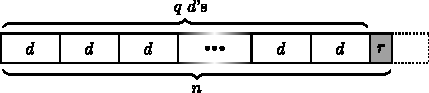
\includegraphics{../graphics/divisionThmProof.pdf}
\]
\begin{question} 
How does the picture above ``prove'' the Division Theorem for positive
integers? How must we change the picture if we allow negative values
for $n$ and $d$?
\end{question}
\QM

\begin{teachingnote}
Highlight uniqueness:  The requirement that  $0 \le r < d$ makes both $d$ and $r$ unique.  Without that requirement, 
many $d$ and $r$ pairs will work.  

The second part of this question is quite challenging.  Some specific examples can help.  
\end{teachingnote}




\begin{activitynote}
Activity \ref{A:CF} complements this section well.  % There Are Many Factors to Consider
\end{activitynote}


\newpage


\begin{problems}
\begin{enumerate}
\item Describe the set of integers. Give some relevant and revealing
  examples/nonexamples.
\item Explain how to model integer addition with pictures or
  items. What relevant properties should your model show?
\item Explain how to model integer multiplication with pictures or
  items. What relevant properties should your model show?
\item Explain what it means for one integer to \textit{divide} another
  integer. Give some relevant and revealing examples/nonexamples.
\item Use the definition of \textit{divides} to decide whether the
  following statements are true or false. In each case, an explanation must 
be given justifying your claim.
\begin{enumerate}
\item $5|30$
\item $7|41$
\item $0|3$
\item $3|0$
\item $6|(2^2\cdot 3^4\cdot 5 \cdot 7)$
\item $1000|(2^7\cdot 3^9\cdot 5^{11}\cdot 17^8)$
\item $6000|(2^{21}\cdot 3^{17}\cdot 5^{89}\cdot 29^{20})$
\end{enumerate}
\item \textit{Incognito's Hall of Shoes} is a shoe store that just
  opened in Myrtle Beach, South Carolina. At the moment, they have 100
  pairs of shoes in stock. At their grand opening 100 customers showed
  up. The first customer tried on every pair of shoes, the second
  customer tried on every 2nd pair, the third customer tried on every
  3rd pair, and so on until the 100th customer, who only tried on the
  last pair of shoes.
\begin{enumerate}
\item Which shoes were tried on by only 1 customer?
\item Which shoes were tried on by exactly 2 customers?
\item Which shoes were tried on by exactly 3 customers?
\item Which shoes were tried on by the most number of customers?
\end{enumerate}
Explain your reasoning.
\item Factor the following integers:
\begin{enumerate}
\item $111$
\item $1234$
\item $2345$
\item $4567$
\item $111111$
\end{enumerate}
In each case, how large a prime must you check before you can be sure
of your answers? Explain your reasoning.
\item Which of the following numbers are prime?  Explain how could deduce whether the numbers are prime in
  as few calculations as possible:
\[
29 \qquad 53 \qquad 101 \qquad 359 \qquad 779 \qquad 839 \qquad 841
\]
In each case, describe precisely which computations are needed and
why those are the only computations needed.
\item Suppose you were only allowed to perform at most $7$
  computations to see if a number is prime. How large a number could
  you check?  Explain your reasoning.
\item Find examples of integers $a$, $b$, and $c$ such that $a \mid
  bc$ but $a\nmid b$ and $a\nmid c$. Explain your reasoning.
\item Can you find at least $5$ composite integers in a row? What
  about at least $6$ composite integers? Can you find $7$?
  What about $n$?  Explain your reasoning. Hint: Consider something
  like $5! = 5\cdot 4 \cdot 3 \cdot 2 \cdot 1$.
\item Use the definition of the \textit{greatest common divisor} to
  find the GCD of each of the pairs below. In each
  case, a detailed argument and explanation must be given justifying
  your claim.
\begin{enumerate}
\item $\gcd(462,1463)$
\item $\gcd(541,4669)$ 
\item $\gcd(10000,2^5\cdot 3^{19}\cdot 5^7\cdot 11^{13})$
\item $\gcd(11111,2^{14}\cdot 7^{21}\cdot 41^{5}\cdot 101)$
\item $\gcd(437^5,8993^3)$
\end{enumerate}

\item Lisa wants to make a new quilt out of $2$ of her favorite
  sheets. To do this, she is going to cut each sheet into as large
  squares as possible while using the entire sheet and using whole
  inch measurements. 
\begin{enumerate}
\item If the first sheet is $72$ inches by $60$ inches what size
  squares should she cut? 
\item If the second sheet is $80$ inches by $75$ inches, what size
  squares should she cut? 
\item How she might sew these squares together? 
\end{enumerate}
Explain your reasoning.
\item Deena and Doug like to feed birds. They want to put 16 cups of
  millet seed and 24 cups of sunflower seeds in their feeder.
\begin{enumerate}
\item How many total scoops of seed (millet or sunflower) are required
  if their scoop holds 1 cup of seed?
\item How many total scoops of seed (millet or sunflower) are required
  if their scoop holds 2 cups of seed?
\item How large should the scoop be if we want to minimize the total
  number of scoops?
\end{enumerate}
Explain your reasoning.
\item Consider the expression:
\[
d\,\begin{tabular}[b]{@{}r@{} r}
$q$ &\, R\,$r$\\ \cline{1-1}
\big)\begin{tabular}[t]{@{}l@{}}
$n$ 
\end{tabular}
\end{tabular}
\qquad\text{where}\qquad
\begin{tabular}{l}
$d$ is the divisor \\
$n$ is the dividend \\
$q$ is the quotient \\
$r$ is the remainder
\end{tabular}
\]
\begin{enumerate}
\item Give $3$ relevant and revealing examples of long division with
  remainders.
\item Given positive integers $d$, $n$, $q$, and $r$ how do you know
  if they leave us with a correct expression above?
\item Given positive integers $d$ and $n$, how many different sets of
  $q$ and $r$ can you find that will leave us with a correct
  expression above?
\item Give $3$ relevant and revealing examples of long division with
  remainders where some of $d$, $n$, $q$, and $r$ are negative.
\item Still allowing some of $d$, $n$, $q$, and $r$ to be negative,
  how do we know if they leave us with a correct expression above?
\end{enumerate}
\item State the \textit{Division Theorem} for integers. Give some
  relevant and revealing examples of this theorem in action.
\item Explain what it means for an integer to \textit{not} divide
  another integer. That is, explain symbolically what it should mean
  to write:
\[
a \nmid b
\]
\item Consider the following:
\begin{align*}
20 \div 8 &= 2 \text{ remainder }4, \\
28 \div 12 &= 2 \text{ remainder }4.
\end{align*}
Is it correct to say that $20 \div 8 = 28 \div 12$? Explain your reasoning.
%\item Explain how if 
%\[
%n = dq_0 + r_0
%\]
%and $r_0> d$, you can find new $q$ and $r$ such that $n = dq+r$ and
%$0\le r< d$.
\item Give a formula for the $n$th even number. Show-off your formula
  with some examples.
\item Give a formula for the $n$th odd number. Show-off your formula
  with some examples.
\item Give a formula for the $n$th multiple of $3$. Show-off your
  formula with some examples.
\item Give a formula for the $n$th multiple of $-7$. Show-off your
  formula with some examples.
\item Give a formula for the $n$th number whose remainder when divided
  by $5$ is $1$. Show-off your formula
  with some examples.

\item Explain the rule
\[
\text{even} + \text{even} = \text{even}
\]
in two different ways. First give an explanation based on
pictures. Second give an explanation based on algebra. Your
explanations must be general, not based on specific examples.
\item Explain the rule
\[
\text{odd} + \text{even} = \text{odd}
\]
in two different ways. First give an explanation based on
pictures. Second give an explanation based on algebra.  Your
explanations must be general, not based on specific examples.
\item Explain the rule
\[
\text{odd} + \text{odd} = \text{even}
\]
in two different ways. First give an explanation based on
pictures. Second give an explanation based on algebra. Your
explanations must be general, not based on specific examples.
\item Explain the rule
\[
\text{even} \cdot \text{even} = \text{even}
\]
in two different ways. First give an explanation based on
pictures. Second give an explanation based on algebra. Your
explanations must be general, not based on specific examples.
\item Explain the rule
\[
\text{odd} \cdot \text{odd} = \text{odd}
\]
in two different ways. First give an explanation based on
pictures. Second give an explanation based on algebra. Your
explanations must be general, not based on specific examples.
\item Explain the rule
\[
\text{odd} \cdot \text{even} = \text{even}
\]
in two different ways. First give an explanation based on
pictures. Second give an explanation based on algebra. Your
explanations must be general, not based on specific examples.
\item Let $a\ge b$ be positive integers with $\gcd(a,b) =1$. Compute
  $\gcd(a +b, a-b)$. Explain your reasoning. Hints: 
\begin{enumerate}
\item Make a chart.
\item If $g|x$ and $g|y$ explain why $g|(x+y)$.
\end{enumerate}
\item Make a chart listing all pairs of positive integers whose
  product is $18$. Do the same for $221$, $462$, and $924$. Use this
  experience to help you explain why when factoring a number $n$, you
  only need to check factors less than or equal to $\sqrt{n}$.
\item \label{P:NNP}Matt is a member of the Ohio State University
  Marching Band. Being rather capable, Matt can take $x$ steps of size
  $y$ inches for all integer values of $x$ and $y$.  If $x$ is
  positive it means \textit{face North and take $x$ steps.} If $x$ is
  negative it means \textit{face South and take $|x|$ steps.} If $y$
  is positive it means your step is a \textit{forward step of $y$
    inches.} If $y$ is negative it means your step \textit{is a
    backward step of $|y|$ inches.}
    \fixnote{We need additional models, e.g., checks and bills, red and black chips. 
    Some of these are incorporated into Activities \ref{A:integerAddition} and \ref{A:integerMultiplication}}
\begin{enumerate}
\item Discuss what the expressions $x \cdot y$ means in this
  context. In particular, what happens if $x = 1$? What if $y=1$?
\item Using the context above, write and solve a word problem that
  demonstrates the rule:
\[
\text{negative}\cdot \text{positive} = \text{negative}
\]
Clearly explain how your problem shows this.
\item Using the context above, write and solve a word problem that
  demonstrates the rule:
\[
\text{negative}\cdot \text{negative} = \text{positive}
\]
Clearly explain how your problem shows this.
\end{enumerate}
\item Stewie decided to count the pennies he had in his piggy bank. He
  decided it would be quicker to count by fives. However, he ended
  with two uncounted pennies. So he tried counting by twos but ended
  up with one uncounted penny. Next he counted by threes and then by
  fours, each time there was one uncounted penny. Though he knew he
  had less than a dollars worth of pennies, and more than 50 cents, he
  still didn't have an exact count. Can you help Stewie out? Explain
  your reasoning.
\end{enumerate}
\end{problems}





\section{The Fundamental Theorem of Arithmetic}\index{Fundamental Theorem!of arithmetic}\label{S:FT}
In the previous section, we found divisors, greatest common divisors, and prime factors of positive integers.  And when we
 found prime factorizations of integers, we used factor trees to organize our work.  

\begin{question}
Jake and Jenna use factor trees to find prime factorizations of the same large number.  Assuming that they don't make any mistakes will their prime factorizations be the same or could they be different?  Explain.  
\end{question}
\QM

Let's try a simpler question. 

\begin{question} If $11 | 50a$, is it true that $11|a$?  Explain and generalize.  
\end{question}
\QM


The following \textit{lemma}\index{lemma} will help us tie these 
ideas together.  What is a lemma, you
ask? A lemma is nothing but a little theorem that helps us solve
another problem.

%Note that a lemma should not be confused with the
%more sour \index{lemon|see{lemma}}\textit{lemon}, as that is something
%different and unrelated to what we are discussing.

\begin{lemma}[Euclid's Lemma]\index{Euclid's Lemma} 
If $p$ is a prime number and $a$ and $b$ are integers
\[
p|ab \qquad\text{implies that} \qquad p | a\text{ or } p|b.
\]
\end{lemma}

We are going to assume Euclid's Lemma without proof (at least for now) because we want to use 
it to prove our fundamental theorem---sometimes called the \textit{Fundamental Theorem of Arithmetic}:

\begin{activitynote}
Activity \ref{A:Prome} complements this section well.  % Prome Factorization
\end{activitynote}

\begin{theorem}[Unique Factorization]\index{Unique Factorization Theorem}\index{Fundamental Theorem!of Arithmetic}
Every integer greater than 1 can be factored uniquely (up to ordering)
into primes.
\end{theorem}

\begin{proof}
Well, if an integer is prime, we are done. If an integer is composite,
then it is divisible by a prime number. Divide and repeat with the
quotient. If our original integer was $n$, we'll eventually get:
\[
n = p_1p_2 \cdots p_m
\]
where some of the $p_i$'s may be duplicates. 

How do we know this factorization is unique? Well, suppose that
\[
n = p_1p_2 \cdots p_m = q_1q_2\cdots q_l
\]
where the $p_i$'s and the $q_j$'s are all prime. By the
definition of ``divides''
\[
p_1 |q_1(q_2\cdots q_l).
\]
So by Euclid's Lemma, $p_1$ must divide either $q_1$ or $(q_2\cdots q_l)$. 
If $p_1 \nmid q_1$, then 
\[
p_1 |q_2(q_3\cdots q_l).
\]
Repeat this
enough times and you will find that $p_1 | q_j$ for one of the $q_j$'s
above, which implies that $p_1 = q_j$. Repeat this process for all 
the $p_i$'s and you see that the factorization is unique.
\end{proof}

\begin{question} 
Huh?! Can you explain what just happened drawing pictures and/or using
symbols as necessary? How do we know the process will terminate?  
Once we see that $p_i | q_j$ for some $j$, how do we know that $p_i = q_j$?
Could you also give some examples?
\end{question}
\QM

\begin{question} 
Thinking about Unique Factorization of the Integers, explain why it
makes sense to exclude $1$ from the prime numbers.
\end{question}
\QM


\begin{question} 
Thinking about Unique Factorization of the Integers, what must be the
case when a number in base ten has units digit of $0$?  What about in other bases?  
\end{question}
\QM

From high school algebra, you have lots of tools for solving equations.  
But in some situations, we are interested only in whole number or integer solutions 
to these equations.  These kinds of equations have a special name:  

\begin{definition}\index{Diophantine equation}
A \textbf{Diophantine equation} is an equation where only integer
solutions are deemed acceptable.
\end{definition}

In this section, we are particularly interested solve \textit{linear Diophantine equations}, that is, equations of the form:
\[
ax + by = c
\]
where $a$, $b$, and $c$ are integers and the only solutions we will
accept are pairs of integers $x$ and $y$.  


\newpage

\begin{problems}

\begin{enumerate}
\item Explain what the GCD of two integers is. Give some relevant and
  revealing examples/nonexamples.
\item Explain what the LCM of two integers is. Give some relevant and
  revealing examples/nonexamples.
\item Consider the Diophantine equation:
\[
15x + 4y = 1
\]
\begin{enumerate}
\item Find a solution to this equation. Explain your reasoning.
\item Compute the slope of the line $15x + 4y = 1$ and write it in
  lowest terms. Show your work.
\item Plot the line determined by $15x + 4y = 1$ on graph paper.
\item Using your plot and the slope of the line, explain how to find
  $10$ more solutions to the Diophantine equation above.
\end{enumerate}
\item Explain why a Diophantine equation 
\[
ax + by = c
\]
has either an infinite number of solutions or zero solutions.
\item Josh owns a box containing beetles and spiders. At the moment,
  there are $46$ legs in the box. How may beetles and spiders are
  currently in the box? Explain your reasoning.
\item How many different ways can thirty coins (nickles, dimes, and
  quarters) be worth five dollars? Explain your reasoning.
\item Lisa collects lizards, beetles and worms. She has more worms
  than lizards and beetles together. Altogether in the collection
  there are twelve heads and twenty-six legs. How many lizards does
  Lisa have?  Explain your reasoning.
\item Can you make exactly \$$5$ with exactly $100$ coins assuming you
  can only use pennies, dimes, and quarters? If so how, if not why
  not?  Explain your reasoning.
\item A merchant purchases a number of horses and bulls for the sum
  of $1770$ talers. He pays $31$ talers for each bull, and $21$ talers
  for each horse. How many bulls and how many horses does the merchant
  buy? Solve this problem, explain what a \textit{taler} is, and
  explain your reasoning---note this problem is an old problem by
  L.\ Euler, it was written in the $1700$'s.
\item A certain person buys hogs, goats, and sheep, totaling $100$
  animals, for $100$ crowns; the hogs cost him $3\frac{1}{2}$ crowns
  a piece, the goats $1\frac{1}{3}$ crowns, and the sheep go for
  $\frac{1}{2}$ crown a piece. How many did this person buy of each?
  Explain your reasoning---note this problem is an old problem from
  \textit{Elements of Algebra} by L.\ Euler, it was written in the
  $1700$'s.
\item How many zeros are at the end of the following numbers:
\begin{enumerate}
\item $2^2 \cdot 5^8 \cdot 7^3\cdot 11^5$
\item $11!$
\item $27!$
\item $99!$
\item $1001!$
\end{enumerate}
In each case, explain your reasoning.
\item Decide whether the following statements are true or false. In
  each case, a detailed argument and explanation must be given
  justifying your claim.
\begin{enumerate}
\item $7|56$
\item $55|11$
\item $3|40$
\item $100 | (2^4\cdot 3^{17} \cdot 5^2\cdot 7)$
\item $5555 | (5^{20}\cdot 7^9\cdot 11^{11}\cdot 13^{23})$ 
\item $3| (3+ 6 + 9 + \cdots +300 + 303)$
\end{enumerate}
\item Suppose that 
\[
(3^5 \cdot 7^9 \cdot 11^x \cdot 13^y) | (3^a \cdot 7^b \cdot 11^{19} \cdot 13^7)
\]
What values of $a$, $b$, $x$ and $y$, make true statements? Explain
your reasoning.
\item Decide whether the following statements are true or false. In
  each case, a detailed argument and explanation must be given
  justifying your claim.
\begin{enumerate}
\item If $7|13a$, then $7|a$.
\item If $6|49a$, then $6|a$. 
\item If $10|65a$, then $10|a$.
\item If $14|22a$, then $14|a$.
\item $54|931^{21}$.
\item $54|810^{33}$.
\end{enumerate}
\item Joanna thinks she can see if a number is divisible by 24 by
  checking to see if it's divisible by 4 and divisible by 6.  She
  claims that if the number is divisible by 4 and by 6, then it must
  be divisible by 24.

Lindsay has a similar divisibility test for 24: She claims that if a
number is divisible by 3 and by 8, then it must be divisible by 24.

Are either correct?  Explain your reasoning.
\item Generalize the problem above.
\item Suppose that you have a huge bag of tickets. On each of the
  tickets is one of the following numbers. 
\[
\{6, 18, 21, 33, 45, 51, 57, 60, 69, 84\}
\]
Could you ever choose some combination of tickets (you can use as many
copies of the same ticket as needed) so that the numbers sum to 7429?
If so, give the correct combination of tickets. If not explain why
not.
\item\label{P:helper} Decide whether the following statements are true
  or false. In each case, a detailed argument and explanation must be
  given justifying your claim.
\begin{enumerate}
\item If $a^2|b^2$, then $a|b$.
\item If $a|b^2$, then $a|b$.
\item If $a|b$ and $\gcd(a,b) = 1$, then $a = 1$.
\end{enumerate}
\item Betsy is factoring the number $24949501$. To do this, she
  divides by successively larger primes. She finds the smallest prime
  divisor to be $499$ with quotient $49999$. At this point she
  stops. Why doesn't she continue? Explain your reasoning.
\item When Ann is half as old as Mary will be when Mary is three times
  as old as Mary is now, Mary will be five times as old as Ann is
  now. Neither Ann nor Mary may vote. How old is Ann? Explain your
  reasoning.
\item If $x^2 = 11\cdot y$, what can you say about $y$? Explain your
  reasoning.
\item If $x^2 = 25\cdot y$, what can you say about $y$? Explain your
  reasoning.
\item When asked how many people were staying at the \textit{Hotel
  Chevalier}, the clerk responded ``The number you seek is the
  smallest positive integer such that dividing by $2$ yields a perfect
  square, and dividing by $3$ yields a perfect cube.'' How many people
  are staying at the hotel? Explain your reasoning.
\end{enumerate}
\end{problems}

\newpage 


\section{The Euclidean Algorithm}\index{Euclidean algorithm}\label{S:EA}
In section~\ref{S:FT}, we assumed Euclid's Lemma and used it to prove the Fundamental 
Theorem of Arithmetic (aka Unique Factorization).  In this section, we backtrack 
to prove Euclid's Lemma.  

\begin{question}
What was Euclid's Lemma?
\end{question}
\QM

\begin{teachingnote}
An important point of this section is to make the student think about
the distributive property. One should try to point out each time
\[
a(x+y) = ax + ay
\]
occurs.
\end{teachingnote}

Up to this point, computing the GCD of two integers required you to
factor both numbers.  This can be difficult to do. The following
algorithm, called the \textit{Euclidean algorithm}, makes finding
GCD's quite easy. With that said, algorithms can be tricky to
explain. Let's try this---study the following calculations, they are
examples of the Euclidean algorithm in action:
\begin{align*}
22 &= \boldsymbol{6}\cdot 3 + \boldsymbol{4}\\ 
\boldsymbol{6} &= \boldsymbol{4}
\cdot 1 + \fbox{$\boldsymbol{2}$}\\ 4 &= 2 \cdot 2 + 0 \qquad 
\fbox{$\therefore \gcd(22,6) = 2$}
\end{align*}

\begin{align*}
33 &= \boldsymbol{24}\cdot 1 + \boldsymbol{9}\\
\boldsymbol{24} &= \boldsymbol{9} \cdot 2 + \boldsymbol{6}\\
\boldsymbol{9} &= \boldsymbol{6} \cdot 1 + \fbox{$\boldsymbol{3}$}\\
6 &= 3 \cdot 2 + 0 \qquad \fbox{$\therefore \gcd(33,24) = 3$} 
\end{align*}

\begin{align*}
42 &= \boldsymbol{16}\cdot 2 + \boldsymbol{10}\\
\boldsymbol{16} &= \boldsymbol{10} \cdot 1 + \boldsymbol{6}\\
\boldsymbol{10} &= \boldsymbol{6} \cdot 1 + \boldsymbol{4}\\
\boldsymbol{6} &= \boldsymbol{4} \cdot 1 + \fbox{$\boldsymbol{2}$}\\
4 &= 2 \cdot 2 + 0 \qquad \fbox{$\therefore \gcd(42,16) = 2$} 
\end{align*}

\begin{question}
Can you describe how to do the Euclidean algorithm?
\end{question}
\QM

\begin{question}
Can you explain why the Euclidean algorithm will always stop? Hint:
Division Theorem.
\end{question}
\QM


\begin{activitynote}
Activity \ref{A:GCDwork} complements this section well.  % Why Does It Work? 
\end{activitynote}


The algorithm demonstrated above is called the \textit{Euclidean
  algorithm} or \textit{Euclid's algorithm} because
Euclid\index{Euclid} uses it several times in Books VII and X of his
book \textit{The Elements}. Donald Knuth\index{Knuth} gives a
description of the Euclidean algorithm in the first volume of his
series of books \textit{The Art of Computer Programming}. Given
integers $m$ and $n$, he describes it as follows:
\begin{quote}
\begin{enumerate} 
\item\label{A:E1} [Find remainder.] Divide $m$ by $n$ and let $r$ be the remainder. (We will have $0\le r< n$.)
\item{[Is it zero?]} If $r=0$, the algorithm terminates; $n$ is the answer.
\item{[Interchange.]} Set $m \leftarrow n$, $n \leftarrow r$, and go
  back to step \ref{A:E1}.
\end{enumerate}
\end{quote}

\begin{question}
What do you think of this description? How does it compare to your
description of the Euclidean algorithm?
\end{question}
\QM

While the Euclidean algorithm is handy and fun, its real power is that
it helps us solve equations. Specifically it helps us solve 
linear Diophantine equations.

Let's study the following calculations:

\begin{tabular}{lr}
\begin{minipage}{15em}
{\begin{align*}
22 &= 6\cdot 3 + 4 &\Leftrightarrow & &  22-6\cdot 3 &= \boldsymbol{4}\\ 
6 &= 4\cdot 1 + 2 &\Leftrightarrow  & &  6 - \boldsymbol{4}\cdot 1 &= 2\\ 
4 &= 2 \cdot 2 + 0 
\end{align*}}
\end{minipage}
&
\begin{minipage}{15em}
{\begin{align*}
6 - 4\cdot 1 &= 2 \\
6 - (22-6\cdot 3)\cdot 1 &= 2 \\
6\cdot 4 + 22(-1) &= 2 
\end{align*}}
\end{minipage} \\
\multicolumn{2}{c}{\fbox{$\therefore 22x + 6y =2$ where $x = -1$ and $y = 4$}}
\end{tabular}

\begin{tabular}{lr}
\begin{minipage}{15em}
{\begin{align*}
33 &= 24\cdot 1 + 9 & \Leftrightarrow & & 33 - 24\cdot 1 &= \boldsymbol{9}\\
24 &= 9 \cdot 2 + 6 & \Leftrightarrow & & 24 - \boldsymbol{9}\cdot 2 &= \boldsymbol{6}\\
9 &= 6 \cdot 1 + 3 & \Leftrightarrow & & 9 - \boldsymbol{6} \cdot 1  &= 3\\
6 &= 3 \cdot 2 + 0  
\end{align*}}
\end{minipage}
&
\begin{minipage}{15em}
{\begin{align*}
9 - 6 \cdot 1  &= 3 \\
9 - (24 - 9\cdot 2) \cdot 1  &= 3 \\
9\cdot 3 +  24\cdot(-1)  &= 3 \\
(33 - 24\cdot 1)\cdot 3 +  24\cdot(-1)  &= 3 \\
33\cdot 3 + 24\cdot (-4) &=3
\end{align*}}
\end{minipage} \\
\multicolumn{2}{c}{\fbox{$\therefore 33x + 24y =3$ where $x = 3$ and $y = -4$}}
\end{tabular}


\begin{question} 
Can you explain how to solve Diophantine equations of the form
\[
ax + by = g
\]
where $g = \gcd(a,b)$?
\end{question}
\QM



The Euclidean algorithm is also useful for theoretical
questions.

\begin{question} 
Given integers $a$ and $b$, what is the smallest positive integer that
can be expressed as
\[
ax + by
\]
where $x$ and $y$ are also integers?
\end{question}

\fixnote{This argument could be improved, as could the corresponding activity, \ref{A:GCDwork}.}

I'm feeling chatty, so I'll take this one. I claim that $g =
\gcd(a,b)$ is the smallest positive integer that can be
expressed as
\[
ax + by
\]
where $x$ and $y$ are integers. How do I know? Well first, the Euclidean algorithm shows that $g$ can be 
expressed as a sum $ax + by$.  (Why?)  

Second, suppose there was
a smaller positive integer, say $s$ where:
\[
ax + by = s
\]
Hmmm\dots but we know that $g|a$ and $g|b$. This means that $g$
divides the left-hand-side of the equation. This means that $g$
divides the right-hand-side of the equation. So $g|s$---but this is
impossible, as $s< g$. Thus $g$ is the smallest integer that can be
expressed as $ax +by$.


\begin{question} Can you now use the Euclidean Algorithm to prove Euclid's Lemma?
\end{question}
\QM


\newpage
\begin{problems}
\begin{enumerate}
\item Explain what a \textit{Diophantine equation} is. Give an example
  and explain why such a thing has real-world applications.
\item Use the Euclidean algorithm to find: $\gcd(671,715)$,
  $\gcd(667,713)$, $\gcd(671,713)$, $\gcd(682,715)$, $\gcd(601,735)$,
  and $\gcd(701,835)$.
\item Explain the advantages of using the Euclidean algorithm to find
  the GCD of two integers over factoring.
\item Find integers $x$ and $y$ satisfying the following Diophantine
  equations:
\begin{enumerate}
\item $671x + 715 y = 11$ 
\item $667x + 713 y = 69$ 
\item $671x + 713 y = 1$
\item $682x + 715 y = 55$
\item $601x + 735 y = 4$
\item $701x + 835 y = 15$
\end{enumerate}
\item Given integers $a$, $b$, and $c$, explain how you know when a
  solution to a Diophantine equation of the form
\[
ax + by = c
\]
exists.
\item Consider the Diophantine equation:
\[
15x + 4y = 1
\]
\begin{enumerate}
\item Use the Euclidean Algorithm to find a solution to this
  equation. Explain your reasoning.
\item Compute the slope of the line $15x + 4y = 1$ and write it in
  lowest terms. Show your work.
\item Plot the line determined by $15x + 4y = 1$ on graph paper.
\item Using your plot and the slope of the line, explain how to find
  $10$ more solutions to the Diophantine equation above.
\end{enumerate}
\item Explain why a Diophantine equation 
\[
ax + by = c
\]
has either an infinite number of solutions or zero solutions.
\end{enumerate}
\end{problems}



\newpage
\section{Rational Numbers}

Once you are familiar with integers, you start to notice something:
Given an integer, it may or may not divide into another integer
evenly. This property is at the heart of our notions of factoring and
primality. Life would be very different if all nonzero integers
divided evenly into one another. With this in mind, we introduce
\textit{rational numbers}.  
\begin{activitynote}
Activities \ref{A:EF} and \ref{A:FO} complement this section well.  
% Picture Models for Equivalent Fractions & Picture Models for Fraction Operations
\end{activitynote}



\begin{definition} 
A \textbf{rational number}\index{rational numbers} can be written as $\dfrac{a}{b}$ where $a\in\Z$, $b\in\Z$, and $b\ne 0$.
\end{definition}

In other words, rational numbers can be written as a fraction of integers, where the denominator is nonzero.
\begin{warning}
Note the words ``can be'' in the definition.  Rational numbers do not have to be represented as fractions.  And fractions are not necessarily rational numbers.  
\end{warning}

\begin{question}
Which of the following numbers are rational?
$$\frac{5}{4}, \qquad 718, \qquad \sqrt{2}, \qquad 2.718, \qquad \frac{22}{7}, \qquad \frac{12}{4}, \qquad \frac{\pi}{3}, \qquad \frac{\sqrt{2}}{\sqrt{8}}, \qquad \frac{1}{43}$$
\end{question}

The set of all \textbf{rational numbers} is denoted by the symbol $\Q$: 
\[
      \Q = \left\{\frac{a}{b}\text{ such that $a\in\Z$ and $b\in\Z$ with $b\ne 0$}\right\}\index{Q@$\Q$}\index{e@$\in$}
\]
The letter $\Q$ stands for the word \textit{quotient}, which should remind us of
fractions.   The funny little ``$\in$'' symbol means ``is in'' or ``is an element of.'' Fancy folks will replace the words \textit{such that} with a colon
``:'' to get:
\[
 \Q = \left\{\frac{a}{b}:\text{$a\in\Z$ and $b\in\Z$ with $b\ne 0$}\right\}
\]


\subsection{Why do People Hate Fractions?}

Why do so many people find fractions difficult? This is a question
worth exploring. We'll guide you through some of the tough spots with
some questions of our own.

\begin{question}
Given a rational number $\dfrac{a}{b}$, come up with three other different rational numbers
that are all equal to $\dfrac{a}{b}$. What features of fractions are we
illustrating?
\end{question}
\QM

\begin{question}
Given two positive rational numbers $\dfrac{a}{b}$ and $\dfrac{c}{d}$, explain how to tell which is greater. What features of fractions are we illustrating?
\end{question}
\QM

\begin{question} 
Given two rational numbers $\dfrac{a}{b}$ and $\dfrac{c}{d}$ with $\dfrac{a}{b} < \dfrac{c}{d}$, explain how one
might find a rational number between them. What features of fractions are we
illustrating?
\end{question}
\QM


\begin{question} 
Dream up counting numbers $a$, $b$, and $c$ such that:
\[
\frac{a/b}{c} = \frac{a}{b/c}
\]
Can you dream up other counting numbers $a'$, $b'$, and $c'$ such that:
\[
\frac{a'/b'}{c'} \neq \frac{a'}{b'/c'}
\]
What features of fractions are we illustrating?
\end{question}
\QM

\begin{question}
Explain how to add two fractions $\dfrac{a}{b}$ and $\dfrac{c}{d}$. What features of
fractions are we illustrating?
\end{question}
\QM


\begin{question} 
Can you come up with any other reasons fractions are difficult?
\end{question}
\QM

\begin{teachingnote}
Two key points of this dialog are: 
\begin{enumerate}
\item Equal fractions have different representations. 
\item It is difficult to compare fractions. 
\end{enumerate}
\end{teachingnote}




\subsection{Basic Meanings of Fractions}
\begin{activitynote}
Activities \ref{A:FlourPower} through \ref{A:CrossSomething} complement this section well. 
%% Flour Power, Picture Yourself Dividing, Cross Something-ing
\end{activitynote}
Like all numbers, fractions have meanings outside of their pure
mathematical existence. Let's see if we can get to the heart of some
of this meaning.\standard{3.NF.1}
\begin{question}
Draw a rectangle. Can you shade $3/8$ of this rectangle? Explain the
steps you took to do this.
\end{question}
\QM


\begin{question}
Draw a rectangle. Given a fraction $a/b$ where $0< a\le b$, explain how
to shade $a/b$ of this rectangle.
\end{question}
\QM


\begin{question}
Draw a rectangle. How could you visualize $8/3$ of this rectangle?
Explain the steps you took to do this.
\end{question}
\QM


\begin{question}
Draw a rectangle. Given a fraction $a/b$ where $0< b< a$, explain how
to visualize $a/b$ of this rectangle.
\end{question}
\QM

\begin{question}
Draw a rectangle.  Can you shade
\[
\frac{3/8}{4}
\]
of this rectangle? Explain the steps you took to do this.
\end{question}
\QM



\newpage

\begin{problems}
\begin{enumerate}
\item Describe the set of rational numbers. Give some relevant and
  revealing examples/nonexamples.
\item What algebraic properties do the rational numbers enjoy that the
  integers do not? Explain your reasoning.
\item What number gives the same result when added to $1/2$ as when
  multiplied by $1/2$. Explain your reasoning.
\item Draw a rectangle to represent a garden. Shade in $3/5$ of the
  garden. Without changing the shading, show why $3/5$ of the garden
  is the same as $12/20$ of the garden. Explain your reasoning.
\item Shade in $2/3$ of the entire picture below:
\[
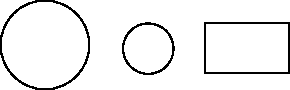
\includegraphics{../graphics/fracPart.pdf}
\]
Explain your reasoning.
\item What fractions could the following picture be illustrating?
\[

\includegraphics{../graphics/whichFrac.pdf}
\]
Explain your reasoning.
\item When Jesse was asked what the $7$ in the fraction $\frac{3}{7}$
  means, Jesse said that the ``$7$'' is the \textit{whole}. Explain
  why this is not completely correct. What is a better description of
  what the ``$7$'' in the fraction $\frac{3}{7}$ means?

\item Find yourself a sheet of paper. Now, suppose that this sheet of
  paper is actually $4/5$ of some imaginary larger sheet of
  paper. 
\begin{itemize}
\item Shade your sheet of paper so that $3/5$ of the larger
  (imaginary) sheet of paper is shaded in. Explain why your shading is
  correct.
\item Explain how this shows that 
\[
\frac{3/5}{4/5} = \frac{3}{4}.
\]
\end{itemize}
\item Try to find the largest rational number smaller than $3/7$.
  Explain your solution or explain why this cannot be done.
\item How many rational numbers are there between $3/4$ and $4/7$?
  Find $3$ of them. Explain your reasoning. 
\item A youthful Bart loved to eat hamburgers. He ate $5/8$ pounds of
  hamburger meat a day. After testing revealed that his blood
  consisted mostly of cholesterol, Bart decided to alter his eating
  habits by cutting his hamburger consumption by $3/4$. How many
  pounds of hamburger a day did Bart eat on his new
  ``low-cholesterol'' diet?  Explain your reasoning.
\item Courtney and Paolo are eating popcorn. Unfortunately, $1/3$rd 
  of the popcorn kernels are poisoned. If Courtney eats exactly $5/16$th 
  of the kernels and Paolo eats exactly $5/13$ths of the kernels, did at 
  least one of them eat a poisoned kernel?  Explain your reasoning.  Also, 
  at least how many kernels of popcorn are in the bowl? Again, explain 
  your reasoning.
\item Best of clocks, how much of the day is past if there remains
  twice two-thirds of what is gone? Explain what this strange question
  is asking and answer the question being sure to explain your
  reasoning---note this is an old problem from the \textit{Greek
    Anthology} compiled by Metrodorus around the year 500.
\item John spent a fifth of his life as a boy growing up, another
  one-sixth of his life in college, one-half of his life as a bookie,
  and has spent the last six years in prison. How old is John now?
  Explain your reasoning
\item Diophantus was a boy for $1/6$th of his life, his beard grew
  after $1/12$ more, he married after $1/7$th more, and a son was born
  five years after his marriage. Alas! After attaining the measure of
  half his father's full life, chill fate took the child. Diophantus
  spent the last four years of his life consoling his grief through
  mathematics. How old was Diophantus when he died?  Explain your
  reasoning---note this is an old problem from the \textit{Greek
    Anthology} compiled by Metrodorus around the year 500.
\item Wandering around my home town (perhaps trying to find my former
  self!), I suddenly realized that I had been in my job for
  one-quarter of my life. Perhaps the melancholia was getting the best
  of me, but I wondered: How long would it be until I had been in my
  job for one-third of my life? Explain your reasoning.
\item In a certain adult condominium complex, $2/3$ of the men are
  married to $3/5$ of the women. Assuming that men are only married to
  women (and vice versa), and that married residents' spouses are also
  residents, what portion of the residents are married? 
\begin{enumerate}
\item Before any computations are done, use common sense to guess the
  solution to this problem.
\item Try to get a feel for this problem by choosing numbers for the
  unknowns and doing some calculations. What do these calculations say
  about your guess?
\item Use algebra to solve the problem.
\end{enumerate}
Explain your reasoning in each step above.

\item Let $a$, $b$, $c$, and $d$ be positive integers such that 
\[
a<b<c<d
\]
Is it true that 
\[
\frac{a}{b}<\frac{c}{d}?
\]
Explain your reasoning.
\item\label{P:CF1} Let $a$, $b$, $c$, and $d$ be positive consecutive
  integers such that
\[
a<b<c<d.
\]
Is it true that 
\[
\frac{a}{b}<\frac{c}{d}?
\]
Explain your reasoning.
\item\label{P:CF2} Let $a$, $b$, $c$, and $d$ be positive consecutive
  integers such that
\[
a<b<c<d.
\]
Is it true that 
\[
\frac{a}{b}<\frac{b}{c}<\frac{c}{d}?
\]
Explain your reasoning.
\item Can you generalize Problem \ref{P:CF1} and Problem \ref{P:CF2}
  above? Explain your reasoning.
\item Let $a$, $b$, $c$, and $d$ be positive integers such that 
\[
\frac{a}{b}<\frac{c}{d}.
\]
Is it true that 
\[
\frac{a}{a+b}<\frac{c}{c+d}?
\]
Explain your reasoning.
\end{enumerate}
\end{problems}

\section{Decimal Representations}

There are two ways that we usually write real numbers that aren't whole numbers:  as fractions and as decimals.  Let's explore the relationship between these two representations of numbers.  

\begin{activitynote}
Activities \ref{A:hundredthsGrids}, \ref{A:Shampoo}, and \ref{A:DecNotNice} are intended for this section. 
% Hundredths Grid
% Shampoo Rinse Repeat
% Decimals Aren't So Nice
\end{activitynote}

\begin{question} How is a ``fraction'' different from a rational number?  
\end{question}
\QM

First, let's work on translating fraction representations into decimal representations.  You probably already know from school that some numbers have decimal representations that end (these are called ``terminating'' decimals) and the rest of them have decimal representations that never end (these are ``non-terminating'').  Try to figure out what it would take for a fraction to have a terminating decimal representation.  

\begin{question}
Write $.465$, $0.72895$, $0.00673$, and $34.062$ as fractions of integers.  What do you notice about terminating decimals when they are written as fractions?  
\end{question}
\QM

\begin{question}
Write $4/5$, $7/16$, $43/20$, and $3/6250$ as decimals.   What about these fractions makes the decimals terminate?
\end{question}
\QM

\begin{question}
Your calculator is not trustworthy for determining whether a number's decimal representation terminates or repeats.  Why?  How can you use your calculator carefully to judge whether a decimal terminates or repeats?  
\end{question}
\QM

In Activity \ref{A:Shampoo}, you separate a bunch of fractions according to whether they appear to have a terminating or non-terminating decimals.  The rational numbers that have a terminating decimals are straighforward to describe, once you see the idea.  The real action (and the intrigue) lies with the non-terminating ones.  

Let's investigate with a fraction that has a non-terminating representation:  4/7.  As you know, 4/7 is the same as ``4 divided by 7.''  So, use long division to find the decimal representation.\standard{7.NS.2d}Bring a pillow, because you already know that it will take an infinite number of steps to complete the work!

Now that you've spent your life doing long division, can you carefully explain why the fraction's non-terminating representation will ``repeat''?  (Hint:  Think about remainders.)  Try a few others, like 2/13, 3/11, or 4/17.  Will the same sort of thing happen with, say, 3457/213678940753?  What can you say about how soon the process will repeat?  

Here are some cool things you can investigate on the side:
\begin{itemize}
\item Some non-terminating decimals have a ``delay'' before they start repeating.  (The most famous one is probably $1/6$.)  I happen to know 1/123750000 will have a delay of 7 places before the repeating starts.  Can you look at a fraction and predict whether it will or will not have a delay (and how long that delay will be)?   
\item What are the restrictions to the sizes of the ``blocks'' for the repeating decimal representation of a rational number?  For example, any fraction with denominator 37 can only possibly repeat in blocks of 1, 2, 3, 4, 6, 9, 12, 18, or 36.
\end{itemize}

Based on the ideas you have explored, you can prove that a non-terminating decimal representation of a rational number must repeat.  Is the converse true?  Can any repeating decimal be written as a fraction?  It turns out indeed to be the case, as can be found by taking advantage of a nice pattern involving the decimals representations of 1/9, 1/99, 1/999, etc., or by noting that each repeating decimal is a ``geometric series,'' as we will explore later.  

Thus, we have it that every rational number can be written as either a terminating or repeating decimal.\standard{8.NS.1}  Can every decimal be written as a fraction?  That is, we have that all fractions are decimals, but are all decimals fractions?  Have we let any decimals out in the cold here?

\begin{question} Describe the decimal representations of 3 ``homemade'' decimals that could never be written as fractions of integers.  Explain your thinking.  Warning:  Do \emph{not} say  $\sqrt{2}$, $\pi$, $e$, or the like, unless you are ready to convince the class that these are not rational numbers.
\end{question}
\QM

\subsection{A Note on Infinite Processes}
Mathematical reasoning often involves ``infinite processes'' in which direct calculation is impossible.\margincomment{This discussion draws heavily on ideas described in \emph{Where Mathematics Comes  From: How the embodied mind brings mathematics into being}  by Lakoff and N\'{u}\~{n}ez (2000).}  Infinite processes become central in calculus, where both differentiation and integration are defined via limits.  These approaches are made rigorous in advanced undergraduate courses, such as Real Analysis.  But infinite processes arise from time to time even in middle grades mathematics, and so it is important that teachers are able to talk about them sensibly and accurately.  Here we explain some key ideas for reasoning about infinite processes.  

First, there is the idea of a process that continues, over and over, without end.  
Here are some examples:
\begin{quote}
\begin{itemize}
\item Perhaps the earliest of these is counting: 1, 2, 3, 4, \dots.  We do not imagine completing the process of counting.  Nonetheless, for any large positive number you name, we can imagine exceeding that number, eventually, if we have enough time.  
\item We can approximate $1/3$ with a sequence, $0.3$, $0.33$, $0.333$, and so on.  We can get as close to $1/3$ as we like by including enough digits.  Note, on the other hand, that it is false to say that $0.3333 = 1/3$ or even $0.3333333333 = 1/3$, because any finite number of digits will miss $1/3$ by an amount that can be calculated precisely.  
\item If we look at a sequence of regular $n$-gons of the same diameter, as $n$ gets large, we can get as close to a circle as we might like.  But for any finite number of sides, the regular $n$-gon will not actually be a circle.  
\end{itemize}
\end{quote}

The above examples use what is sometimes called \emph{potential infinity}, for in none of the cases do we actually complete the process, and we do not need to.  We imagine these things as going on ``forever,'' and a process that goes on forever never ends.  

But the interesting uses of infinity in mathematics involve \emph{actual infinity}.  
\begin{question}
In each of the above examples, what would happen if the process could end?
\end{question}
\QM

In order to conceptualize actual infinity, we imagine, metaphorically, that the process \emph{does} end.  In a literal sense, an infinite process cannot end, but through the use of metaphor, we consider what would happen if the process were to end.  And with the help of intuitions about completed processes, we then infer the ``ultimate result'' of the completed infinite process.    

With the metaphor of actual infinity, counting yields the infinite set of counting numbers, $\N$.  All of them.  In the repeating decimal for $1/3$, we get an exact decimal representation, so that $0.33333\ldots = 1/3$.  Exactly.  And in the case of the regular $n$-gon with an infinite number of sides, we get a circle.  Perfectly.  

\begin{warning}
With the metaphor of actual infinity, it is \emph{false} to say that $0.3333\ldots$ never gets to $1/3$ because the dots imply that the infinite process has been completed.  Although any finite number of digits fails reach $1/3$, an infinite number of digits reaches $1/3$ exactly:  The error has gone to 0.  
\end{warning}

In summary, reasoning about infinite processes involves the following steps:  
\begin{quote}
\begin{enumerate}
\item Describing the finite process carefully and accurately;
\item Considering the process to go on forever, and describing how the result can get arbitrarily close to some goal;
\item Imagining that the infinite process has been completed; and
\item Reasoning about the ``ultimate result'' of the infinite process.
\end{enumerate}
\end{quote}

For some infinite processes, it is quite helpful in the second and fourth steps to talk about the ``error,'' which is to say how much the finite process falls short of the ultimate goal, and then to argue that the error becomes arbitrarily small (i.e., it goes to 0). 

\vspace{0.2in}

Happy infinite reasoning!   

\newpage

\begin{problems}
\begin{enumerate}

\subsection*{Exercises}

\item What does $3.417$ mean in the base-ten place-value system?  Using the rectangle below as $1$, draw a picture the illustrates the place-value meaning of $3.417$.  Draw as accurately as you can, indicating how the picture would be drawn perfectly (if you could).  Indicate whether your model is primarily about length, area, or something else.  

\vspace{.5cm}
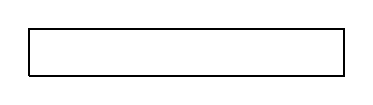
\begin{tikzpicture}
\draw [thick] (0,0) -- (4,0) -- (4,.6) -- (0,.6) -- (0,0);
\end{tikzpicture}

\item Plot $3.417$ on each of the following number lines, zooming in to show how to make the placement more accurate at each step.  Draw dotted curves (as shown) to indicate where the zooming takes place, and label the large tick marks on each number line.  
\vspace{0.5cm}

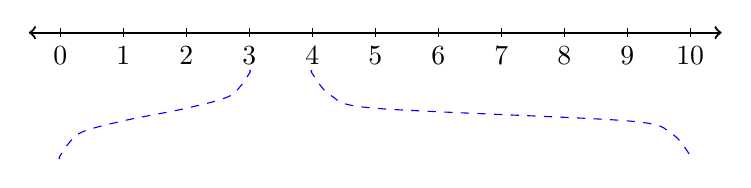
\begin{tikzpicture}[scale=0.8]
% a straight line segment
\draw [thick, <->] (-0.5,0) -- (10.5,0);
% the ticks and their labels
\foreach \x  in {0,...,10}
  \draw[xshift=\x cm] (0pt,2pt) -- (0pt,-2pt) node[below,fill=white] {\the\numexpr\x \relax};

\draw[dashed, blue] plot [smooth] coordinates{(3,-0.6) (3,-0.65) (2.7,-1) (2,-1.2) (1,-1.4)  (0.3,-1.6) (0,-1.95) (0,-2)};
\draw[dashed, blue] plot [smooth] coordinates{(4,-0.6) (4,-0.65) (4.3,-1) (5,-1.2) (9,-1.4)  (9.7,-1.6) (10,-1.95) (10,-2)};
\end{tikzpicture}

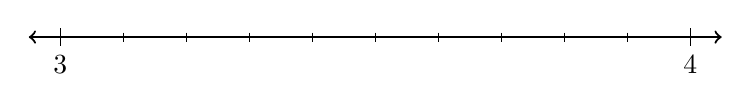
\begin{tikzpicture}[scale=0.8]
% a straight line segment
\draw [thick, <->] (-0.5,0) -- (10.5,0);
% the ticks and their labels
 \draw[xshift=0 cm] (0pt,4pt) -- (0pt,-4pt) node[below,fill=white] {\the\numexpr3 \relax};
\foreach \x  in {1,...,9}
  \draw[xshift=\x cm] (0pt,2pt) -- (0pt,-2pt);
 \draw[xshift=10 cm] (0pt,4pt) -- (0pt,-4pt) node[below,fill=white] {\the\numexpr4 \relax};
\end{tikzpicture}

\vspace{0.8cm}

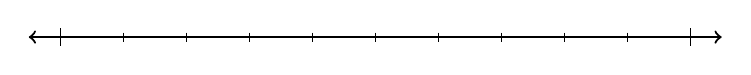
\begin{tikzpicture}[scale=0.8]
% a straight line segment
\draw [thick, <->] (-0.5,0) -- (10.5,0);
% the ticks and their labels
 \draw[xshift=0 cm] (0pt,4pt) -- (0pt,-4pt) ; 
\foreach \x  in {1,...,9}
  \draw[xshift=\x cm] (0pt,2pt) -- (0pt,-2pt);
 \draw[xshift=10 cm] (0pt,4pt) -- (0pt,-4pt) ; 
\end{tikzpicture}

\vspace{1.2cm}

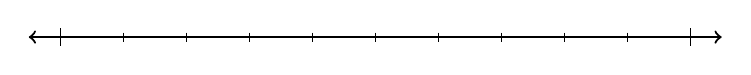
\begin{tikzpicture}[scale=0.8]
% a straight line segment
\draw [thick, <->] (-0.5,0) -- (10.5,0);
% the ticks and their labels
 \draw[xshift=0 cm] (0pt,4pt) -- (0pt,-4pt) ; 
\foreach \x  in {1,...,9}
  \draw[xshift=\x cm] (0pt,2pt) -- (0pt,-2pt);
 \draw[xshift=10 cm] (0pt,4pt) -- (0pt,-4pt) ; 
\end{tikzpicture}

\vspace{0.4cm}

\item How would your plotted points in the four number lines have been different if the number had been 341.7?  What about 0.003417?  Or 34,170,000?   What does your answer say about the consistent structure of the base-ten place value system?  (Hint:  In each number, how does the meaning of the 4 compare to the meaning of the 1 to its right?   How does the meaning of the 4 compare to the meaning of the 3 to its left?)  

\item How would your plotted points in the four number lines have been different if the number had been 3.41708?  What about 3.41708667999?  Explain.  

\item You should know or be able to figure out (in your head) decimal equivalents of fractions with many small  or ``nice'' denominators (i.e., 2, 3, 4, 5, 6, 8, 9, 10, 11, 12, 16, 20, 25, 30, 40, and 50).  Describe how to figure out quickly any that you might forget.  

\item Here is a nice relationship between twelfths and eighths:  $1/8\approx 0.12$ and $1/12\approx 0.08$.  Find other such pairs, and explain why the pairs ``work'' this way.   

\item Compare the decimal representations of $\frac{1}{7}$, $\frac{2}{7}$, $\frac{3}{7}$, $\frac{4}{7}$, $\frac{5}{7}$, and  $\frac{6}{7}$.
\begin{enumerate}  
\item Notice that the repeating digits always appear in the same order.  Explain why this is the case.
\item Suppose you are able to remember the decimal representation of $\frac{1}{7}$.  Explain how to use that to write quickly the decimal representation of any of the other sevenths.  
\end{enumerate}

\item 
Compare the decimal representations of $\frac{1}{13}$, $\frac{2}{13}$, \dots,  $\frac{12}{13}$.  
\begin{enumerate}  
\item Describe carefully how the order of the digits is somewhat like and also different from what you noticed for sevenths.  
\item Explain why the decimal representations of thirteenths work as you described.
\end{enumerate}

\item Without a calculator, predict whether the decimal representations of the following numbers will terminate or not.  For those that terminate, predict the number of decimal places.  
\begin{enumerate}
\item $\dfrac{13}{400}$
\item $\dfrac{11}{70}$
\item $\dfrac{21}{70}$
\item $\dfrac{27}{6250}$
\item $\dfrac{23}{2^7\cdot 5^2}$
\item $\dfrac{23}{2^7\cdot 5^2\cdot 11}$
\item $\dfrac{22}{2^7\cdot 5^2\cdot 11}$
\end{enumerate}

\item The clearest way to demonstrate that a number is rational is to show that it satisfies the definition.  (What is the definition of a rational number?)  Show that the following numbers are rational:  
\begin{enumerate}
\item $0.\overline{324}$
\item $15.\overline{324}$
\item $0.15\overline{324}$
\item $0.2\overline{5643}$
\end{enumerate}


\subsection*{Generalizations}
\item Use long division to explain why the decimal representation of a rational number must either terminate or repeat.

\item Suppose $\frac{m}{n}$ is a rational number in lowest terms.  If the number's decimal representation terminates, what can you conclude about $m$ and about $n$?  Explain.  

\item Suppose $\frac{m}{n}$ is a rational number in lowest terms.  If you know the number's decimal representation repeats, what can you conclude about the number of repeating digits?  Explain.  

\item You have seen three types of decimal representations for rational numbers between 0 and 1:  terminating, repeating, and delayed-repeating.  Suppose that $m$ and $n$ are counting numbers with no common factors and $m<n$.  Explain why the type of decimal representation of $\frac{m}{n}$ depends only on $n$ and not on $m$.  Hint:  Consider the three types separately.  

\subsection*{Explorations}

\item The rational number $\frac{1}{19}$ has decimal representation $0.\overline{052631578947368421}$.  To verify this, your calculator is unlikely to display enough digits, and long division would be quite tedious.  Devise a method for ``piecing together'' this decimal representation in ``chunks,'' using your calculator.  Then use the method to compute the decimal representation of $\frac{7}{23}$.  Be sure to indicate how you know that it repeats as you claim.  

\item Given a prime number $p$, find the smallest positive integer $n$ so that $p$ divides $10^n-1$, or explain why there is no such integer $n$.  
\begin{enumerate}
\item Do this for all primes less than 15, and also for the primes 37, 41, 73, and 101.
\item For each prime, compare the $n$ you found with the number of repeating digits in the decimal representation of $\frac{1}{p}$.  
Make a conjecture about what you notice.  Provide a brief explanation of why your conjecture ought to be true. 
\end{enumerate}

% In the following two problems, keep in mind that you are trying to explain arithmetic of decimals, which you will teach in grade 5.  
% So your explanations should NOT USE arithmetic of decimals.  Use fractions and the meanings of 
% decimals instead.  And it would be better if you do not use %negative exponents, which is in grade 8.

\item Explain $2.7\times 3.4$ in \textbf{two different ways}.  Be sure your explanations address two key questions:  (i) Why can you almost ignore the decimal point and multiply as though the digits described whole numbers?  And (ii) How do you know where to place the decimal point in the result?  Here are some ideas:  
\begin{itemize}
\item Use behind the scenes algebra to explain why the digits in the  $27\times 34$ should be the same as the digits in the desired product $2.7\times 3.4$.  
\item Convert the decimals to fractions, compute the product of the fractions, and then convert the result to a decimal.  
\item Use the picture below to compute $2.7\times 3.4$ with neither an algorithm nor a calculator.  Explain your reasoning.  
\[
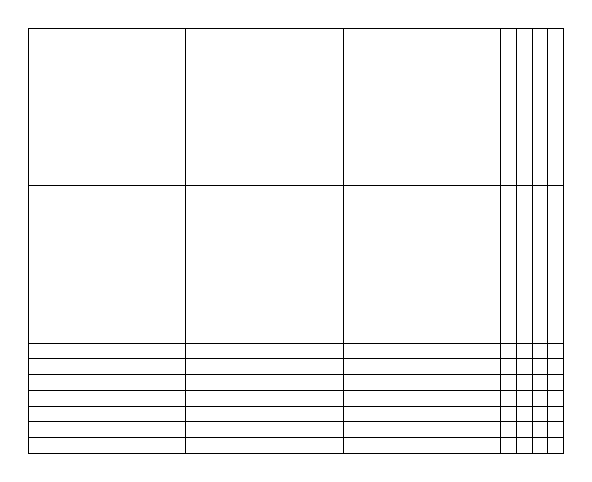
\begin{tikzpicture}[scale=2]
%\draw [line width=0.1pt,gray!30,step=1mm] (0,0) grid (3.4,2.7);
%\draw [help lines] (0,0) grid (3.4,2.7);
\draw (0,0) grid (3,2);
\draw [xstep=1cm,ystep=1mm] (0,-0.7) grid (3,0);
\draw [xstep=1mm,ystep=1cm] (3,0) grid (3.4,2);
\draw [xstep=1mm,ystep=1mm] (3,-0.7) grid (3.4,0);
\end{tikzpicture}
\]
\item Explain why the above picture can also represent $27\times 34$.  Explain the lengths and areas for both calculations.  

\end{itemize}

\item Explain $3.96\div 2.4$ in \textbf{two different ways}.  Be sure your explanations address two key questions:  (i) Why can you almost ignore the decimal point and divide as though the digits described whole numbers?  And (ii) How do you know where to place the decimal point in the result?  Here are some ideas:  
\begin{itemize}
\item Use the measurement model of division to reason how many groups of size $2.4$ are in $3.96$.
\item Use bundles or base ten blocks where the single stick or unit block represents a quantity other than 1.  
\item Multiply both the dividend and the divisor by a suitable power of 10 and then divide.  
\item Convert both decimals to fractions, divide the fractions, then convert the result back to a decimal.  
\item Divide $396$ by $24$ and then use estimation to place the decimal point.  
\end{itemize}

\end{enumerate}
\end{problems}




\setcounter{chapter}{2}
%\input{../chapters/ratioFront}

\appendix

\renewcommand{\theenumi}{$(\mathrm{\alph{enumi}})$}
\renewcommand{\labelenumi}{\theenumi}
\chapter{Supplemental Activities}



% Put activities here 



%\setcounter{page}{1}

\setcounter{section}{19}
%\newpage
\section{Poor Old Horatio}\label{A:ratios}


%  If you find that you want to write an equation, explain why the equation makes sense, and explain the steps in your solution process.  

\begin{prob}
A shade of orange is made by mixing 3 parts red paint with 5 parts
yellow paint.  Sam says we can add 4 cups of each color of paint and
maintain the same color.  Fred says we can quadruple both 3 and 5 and
get the same color.  
\begin{enumerate}
\item Who (if either or both) is correct?  Explain your reasoning.
\vspace{0.35in}

\item Use a table like the one below to show other paint mixtures that are the desired shade of orange. 
\[{\renewcommand{\arraystretch}{2}
\begin{tabular}{|c||c|c|c|c|c|c|c|c|}\hline
Red  &  3 &\rule[7mm]{12mm}{0mm} & \rule[7mm]{12mm}{0mm} & \rule[7mm]{12mm}{0mm}  & \rule[7mm]{12mm}{0mm}
 & \rule[7mm]{12mm}{0mm} & \rule[7mm]{12mm}{0mm} & \rule[7mm]{12mm}{0mm}   \\ \hline
Yellow & 5 &  &  &  & & & & \\ \hline
           &   &  &  &  & & & & \\ \hline
\end{tabular}}
\]
\end{enumerate}
\end{prob}


\begin{prob}
If we wanted to make the same orange paint but were required to use 73 cups of yellow paint, how
many cups of red paint would we need?  Explain your reasoning.  
\vspace{0.1in} 
\[{\renewcommand{\arraystretch}{2}
\begin{tabular}{|c||c|c|c|c|c|}\hline
Red  &  3 &\rule[7mm]{12mm}{0mm} &\rule[7mm]{12mm}{0mm} & \rule[7mm]{12mm}{0mm}  & \rule[7mm]{12mm}{0mm}   \\ \hline
Yellow & 5 &  &  &  & \\ \hline
           &   &   &    &  &  \\ \hline
\end{tabular}}
\]
\vspace{0.1in} 
\end{prob}


%\vspace{0.25in}

\begin{prob}
If we wanted to make the same orange paint but were required to use 56 cups of red paint, how
many cups of yellow paint would we need?  Explain your reasoning.  
\vspace{0.1in} 
\[{\renewcommand{\arraystretch}{2}
\begin{tabular}{|c||c|c|c|c|c|}\hline
Red  &  3 &\rule[7mm]{12mm}{0mm} &\rule[7mm]{12mm}{0mm} & \rule[7mm]{12mm}{0mm}  & \rule[7mm]{12mm}{0mm}   \\ \hline
Yellow & 5 &  &  &  & \\ \hline
           &   &   &    &  &  \\ \hline
\end{tabular}}
\]
\vspace{0.1in} 
\end{prob}

%\vspace{0.25in}

%\begin{prob}
%Is ``cross-multiplication''a legitimate way to solve the equations
%arising from this sort of problem---be sure to think of the weird
%units that are generated by doing so.  What good is this kooky method?
%What exactly is one doing when they ``cross-multiply'' and what type
%of problem does it solve?
%\end{prob}

\begin{prob}
Generalize your approaches to the previous problems.  
\begin{enumerate}
\item Give a general formula for computing how much red paint
is needed when $y$ cups of yellow paint is used.   
\item Give a general formula for computing how much yellow paint
 is needed when $r$ cups of red paint is used. 
\end{enumerate}
\vspace{0.1in} 
\[{\renewcommand{\arraystretch}{2}
\begin{tabular}{|c||c|c|c|c|c|}\hline
Red  &  3 &  &  &  &   \\ \hline
Yellow & 5  &\rule[7mm]{12mm}{0mm} &\rule[7mm]{12mm}{0mm} & \rule[7mm]{12mm}{0mm} & \rule[7mm]{12mm}{0mm}  \\ \hline
          &    &  &  &   &  \\ \hline
\end{tabular}}
\]
\vspace{0.1in} 
\end{prob}

\begin{prob}
Now suppose we want to make a \textbf{different shade} of orange, this time made with $\frac{3}{4}$ cup of red paint and $\frac{2}{3}$ cup of yellow paint.  How many cups of each color do you need in order to make 15 cups of the mixture?  Use the table below.  
\vspace{0.1in} 
\[{\renewcommand{\arraystretch}{2}
\begin{tabular}{|c||c|c|c|c|c|}\hline
Red  &  $\frac{3}{4}$ &  &  &  &   \\ \hline
Yellow & $\frac{2}{3}$  &\rule[7mm]{12mm}{0mm} &\rule[7mm]{12mm}{0mm} & \rule[7mm]{12mm}{0mm} & \rule[7mm]{12mm}{0mm}  \\ \hline
          &  & $17$  & $1$ & $15$   &  \\ \hline
\end{tabular}}
\]
\vspace{0.1in} 
\end{prob}

\begin{teachingnote}
Call attention to part/part vs. part/whole approaches. 
\end{teachingnote}

\begin{prob}
In proportional reasoning problems, a \emph{unit rate} describes the amount of one quantity for 1 unit of another quantity.  
\begin{enumerate}
\item What are the units for the various numbers in these problems?  
\item Identify some unit rates in this activity.  
\item In solving the above problems, it is likely that you or your classmates use strategies that made use of unit rates on the way to your solution.  Explain why this strategy is sometimes called \emph{going through one}.
\end{enumerate}
\end{prob}

\fixnote{Revise these problems drawn from Beckmann.  Use dollars/pound, or meters/second, etc.}

\begin{prob}
If $2\frac{1}{2}$ pints of jelly fills $3\frac{1}{2}$ jars, then how many jars will you need for 12 pints of jelly?  (Assume the jars are all the same size.)  If the last jar is not totally full, indicate how full it will be.  
\vspace{0.1in} 
\[{\renewcommand{\arraystretch}{2}
\begin{tabular}{|c||c|c|c|c|c|c|c|c|}\hline
Jelly  &  \rule[7mm]{12mm}{0mm} &\rule[7mm]{12mm}{0mm} & \rule[7mm]{12mm}{0mm} & \rule[7mm]{12mm}{0mm}  
 & \rule[7mm]{12mm}{0mm} & \rule[7mm]{12mm}{0mm} & \rule[7mm]{12mm}{0mm} & \rule[7mm]{12mm}{0mm}   \\ \hline
Jars &  &  &  &  & & & & \\ \hline
           &  &  &  &  & & & & \\ \hline
\end{tabular}}
\]
\vspace{0.1in} 
\end{prob}




%\setcounter{section}{22}
%\newpage
\section{The Triathlete}\label{A:Triathlete}

\begin{prob} 
On Friday afternoon, just as Laine got off the bus, she realized that she had left her bicycle at school.  In order to have her bicycle at home for the weekend, she decided to run to school and then ride her bike back home.  If she averaged 6 mph running and 12 mph on her bike, what was her average speed for the round trip?  Explain your reasoning. 
\end{prob}

\begin{teachingnote}
A key idea here is that the average speed is independent of the distance.  Here are several ways that students can solve it: 
\begin{itemize}
\item Pick a distance, say 12 miles.  Then running to school will take 2 hours, and biking back home will take 1 hour.  That's a total of 24 miles in 3 hours, or an average of 8 mph.  
\item Let the distance be $d$.  Then running to school will take $\frac{d}{6}$ hours, and biking back home will take $\frac{d}{12}$ hours.  The total distance is $2d$.  So the average rate is 

$$\frac{2d}{\frac{d}{6}+\frac{d}{12}}=\frac{2}{\frac{1}{6}+\frac{1}{12}}=\frac{2}{\frac{3}{12}}=\frac{2}{\frac{1}{4}}=8 \text{ mph}$$
Notice that the $d$ factors out of both the numerator and the denominator (and hence cancels), which shows that the average speed is independent of the distance.  

Notice also that this calculation can be expressed as a different kind of average:  $$\frac{\frac{1}{6}+\frac{1}{12}}{2}=\frac{1}{8}$$
This average is called the \emph{harmonic mean}.  Specifically, 8 is the harmonic mean of 6 and 12 because it is the reciprocal of the average of their reciprocals.  (Math 1165 students do not need to know this language.)
\item Sometimes is helpful to think of speed as ``time per distance,'' which is the reciprocal of ``distance per time.''  In this problem, we can reason that Lanie runs a ``ten-minute mile" as follows:  Her speed of 6 mph would be $\frac{1}{6}$ hour/mile, which is the same as 10 min/mile.  Similarly, she bikes at 5 min/mile.  With this insight, we can cut the distance between home and school into 1-mile pieces and reason that she will take 10 minutes to run each mile and 5 minutes to bike the same mile on the way home.  That would be 15 minutes for both directions (2 miles), for an average speed of 7.5 min/mile, which is the same as 8 mph.  
\item Another way of thinking about these kinds of problems is as weighted averages.  For example, because the distances are the same, Laine will spend twice as much time running (i.e., at half the speed) as she spends on her bike.  Thus, we can weight the 6 mph running speed twice and the 12 mph biking speed just once, as follows:  
$$\textrm{Average speed }= \frac{2\cdot6 + 12}{3} = 8.$$
Notice we divide by 3 because that is the sum of the weights.  The same reasoning can work even when the numbers are more challenging.  
\end{itemize}
\end{teachingnote}

\begin{prob}
On Saturday, Laine completed a workout in which she split the time evenly between running and cycling.  If she again averaged 6 mph running and 12 mph on her bike, what was her average speed for the workout?  Explain your reasoning. 
\end{prob}

\begin{teachingnote}
Here the naive calculations works:  The average speed is the average of the two speeds, so the answer is $\frac{6+12}{2}=9$ mph.  But we should be clear why this works.  Here are two approaches: 
\begin{itemize}
\item Pick a time, say 1 hour, to spend on each activity.  Lanie will run 6 miles in 1 hour and will bike 12 miles in 1 hour.  That will be 18 miles in 2 hours, or an average of 9 mph.  This will work, of course, for every hour of activity, which suggests that the result is independent of time.  
\item Algebra:  Let the $t$ represent the time spent on each activity.  The distance running will be $6t$, the distance biking will be $12t$, and the total time will be $2t$.  So the average speed will be $$\frac{6t+12t}{2t}=\frac{18t}{2t}=9 \text{ mph.}$$  
Notice the common factor of $t$ cancels, which shows that the average speed is independent of the time.  
\end{itemize}
\end{teachingnote}

\begin{prob}
Why was her average speed on Saturday different from her average speed on Friday?  Can you reason, without computation, which average speed should be faster?  
\end{prob}

\begin{teachingnote}
One approach:  When the times are the same, the average will be midway between the two speeds.  When the distances are the same, in contrast, she will spend more time traveling at the slower speed than at the faster speed, so the average will be closer to the slower speed, which implies that the same-distance average is slower than the same-time average.  
\end{teachingnote}

\begin{prob} On Sunday, Laine's workout included swimming.  Assuming that she can swim at an average speed of 2 mph, describe two running-cycling-swimming workouts, one similar to Friday's scenario (same distance) and a second similar to Saturday's (same time).  Compute the average speed for each and explain your reasoning.  
\end{prob}

\begin{teachingnote}
Same distance (a la Friday):  

$$\text{Average speed } = \frac{3d}{\frac{d}{2}+\frac{d}{6}+\frac{d}{12}}=\frac{3}{\frac{1}{2}+\frac{1}{6}+\frac{1}{12}}=\frac{3}{\frac{9}{12}}=\frac{3}{\frac{3}{4}}=4  \text{ mph.}$$

Same time (a la Saturday):  $$\text{Average speed } = \frac{2t+6t+12t}{3t}=\frac{20t}{3t}=6\frac{1}{3} \text{ mph.}$$
\end{teachingnote}

\begin{prob}
Which of the workout scenarios (same distance or same time) most closely resembles an actual triathlon?  Why do you think that is the case?
\end{prob}

\begin{teachingnote}
In actual triathlons, the running distances are much shorter than the biking distances, and the swimming distances are much shorter still.  It would not be reasonable to swim any reasonable biking distance.  So the ``same time'' scenario is closer.  But in reality, the swimming times are quite a bit shorter than the running and biking times.  
\end{teachingnote}

\begin{prob}
After two months of intense training, Laine is able to average $s$ mph swimming, $r$ mph running, and $c$ mph cycling.  Again describe two running-cycling-swimming workouts, one similar to each of the two original scenarios, and compute her average speeds.     
\end{prob}

\begin{teachingnote}
Same distance (a la Friday):  

$$\text{Average speed } = \frac{3d}{\frac{d}{s}+\frac{d}{r}+\frac{d}{c}}=\frac{3}{\frac{1}{s}+\frac{1}{r}+\frac{1}{c}}$$

Same time (a la Saturday):  $$\text{Average speed } = \frac{st+rt+ct}{3t}=\frac{(s+r+c)t}{3t}=\frac{s+r+c}{3}$$
\end{teachingnote}


%\setcounter{page}{1}

\setcounter{section}{53}

%\newpage
\section{Hundredths Grids for Rational Numbers}\label{A:hundredthsGrids}

%% Use tikz to generate the graphics

When a $10\times 10$ square is taken to be $1$ whole, it can be used as a ``hundredths grid'' 
to represent fractions and decimals between $0$ and $1$.\margincomment{For example, one of the grids below 
is shaded to represent $\frac{21}{100}$.}

\begin{prob}
Shade the hundredths grids to show each of the following fractions.  Then use your shading to determine a decimal equivalent for each fraction.  
\begin{center}
\hfill (a) $\frac{3}{20}$ \hfill (b) $\frac{1}{8}$ \hfill (c) $\frac{1}{6}$ \hfill (d) $\frac{7}{12}$ \hfill
\end{center}

\begin{fullwidth}\em\em\quad
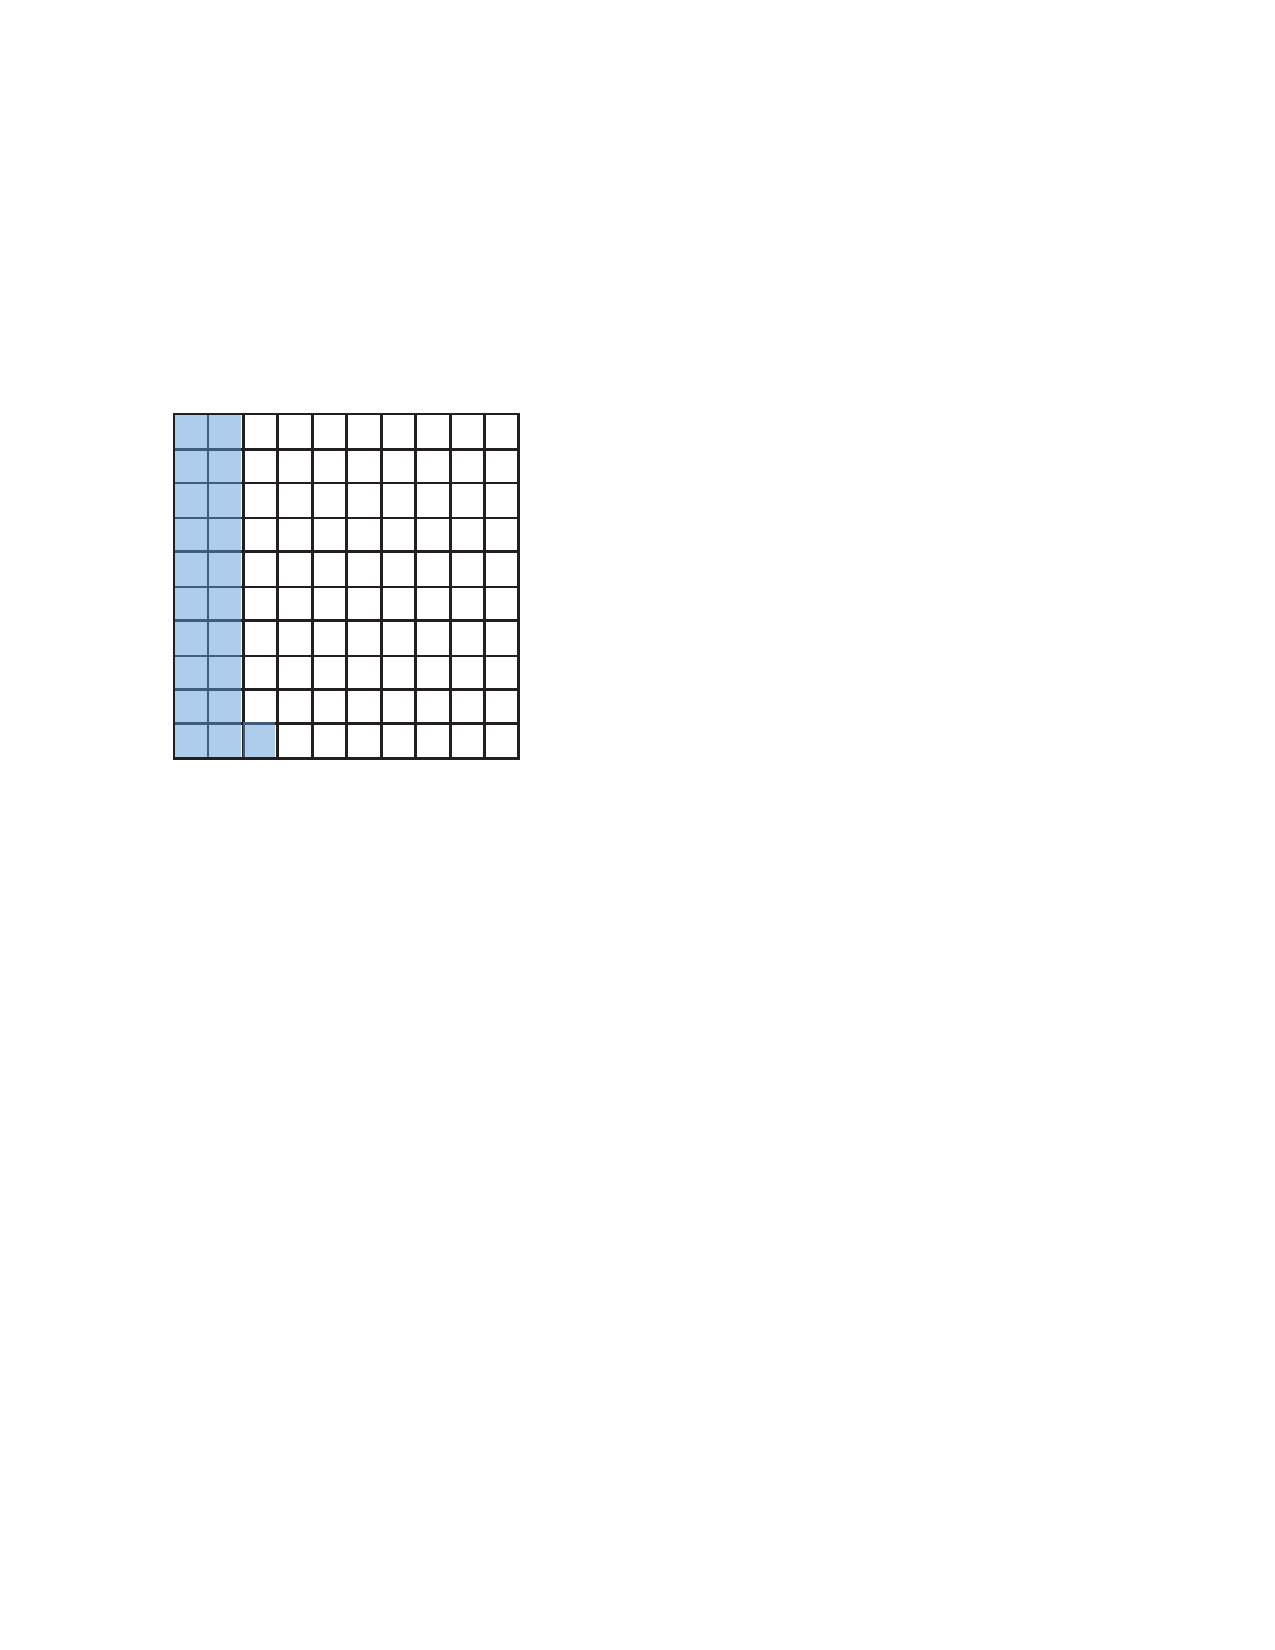
\includegraphics{../graphics/hundredthsGridSample}\quad
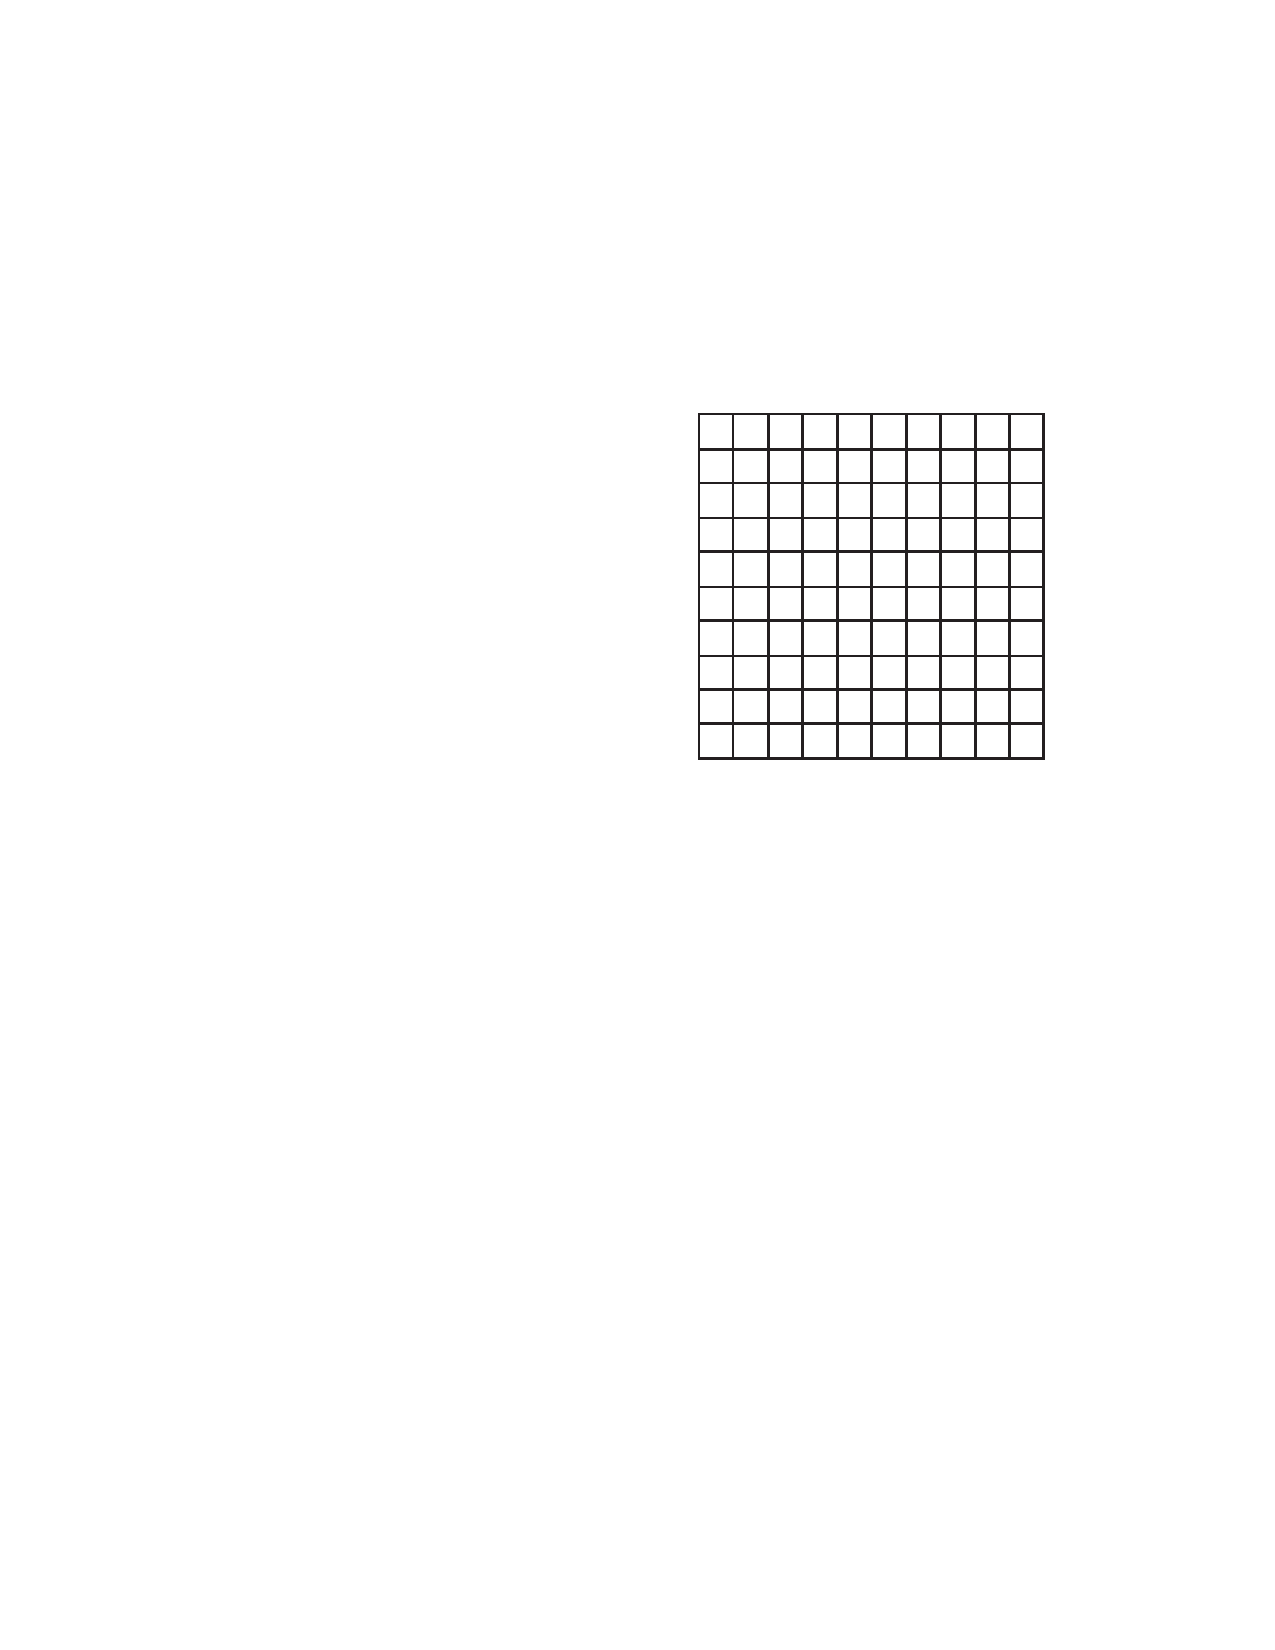
\includegraphics{../graphics/hundredthsGrid}\quad
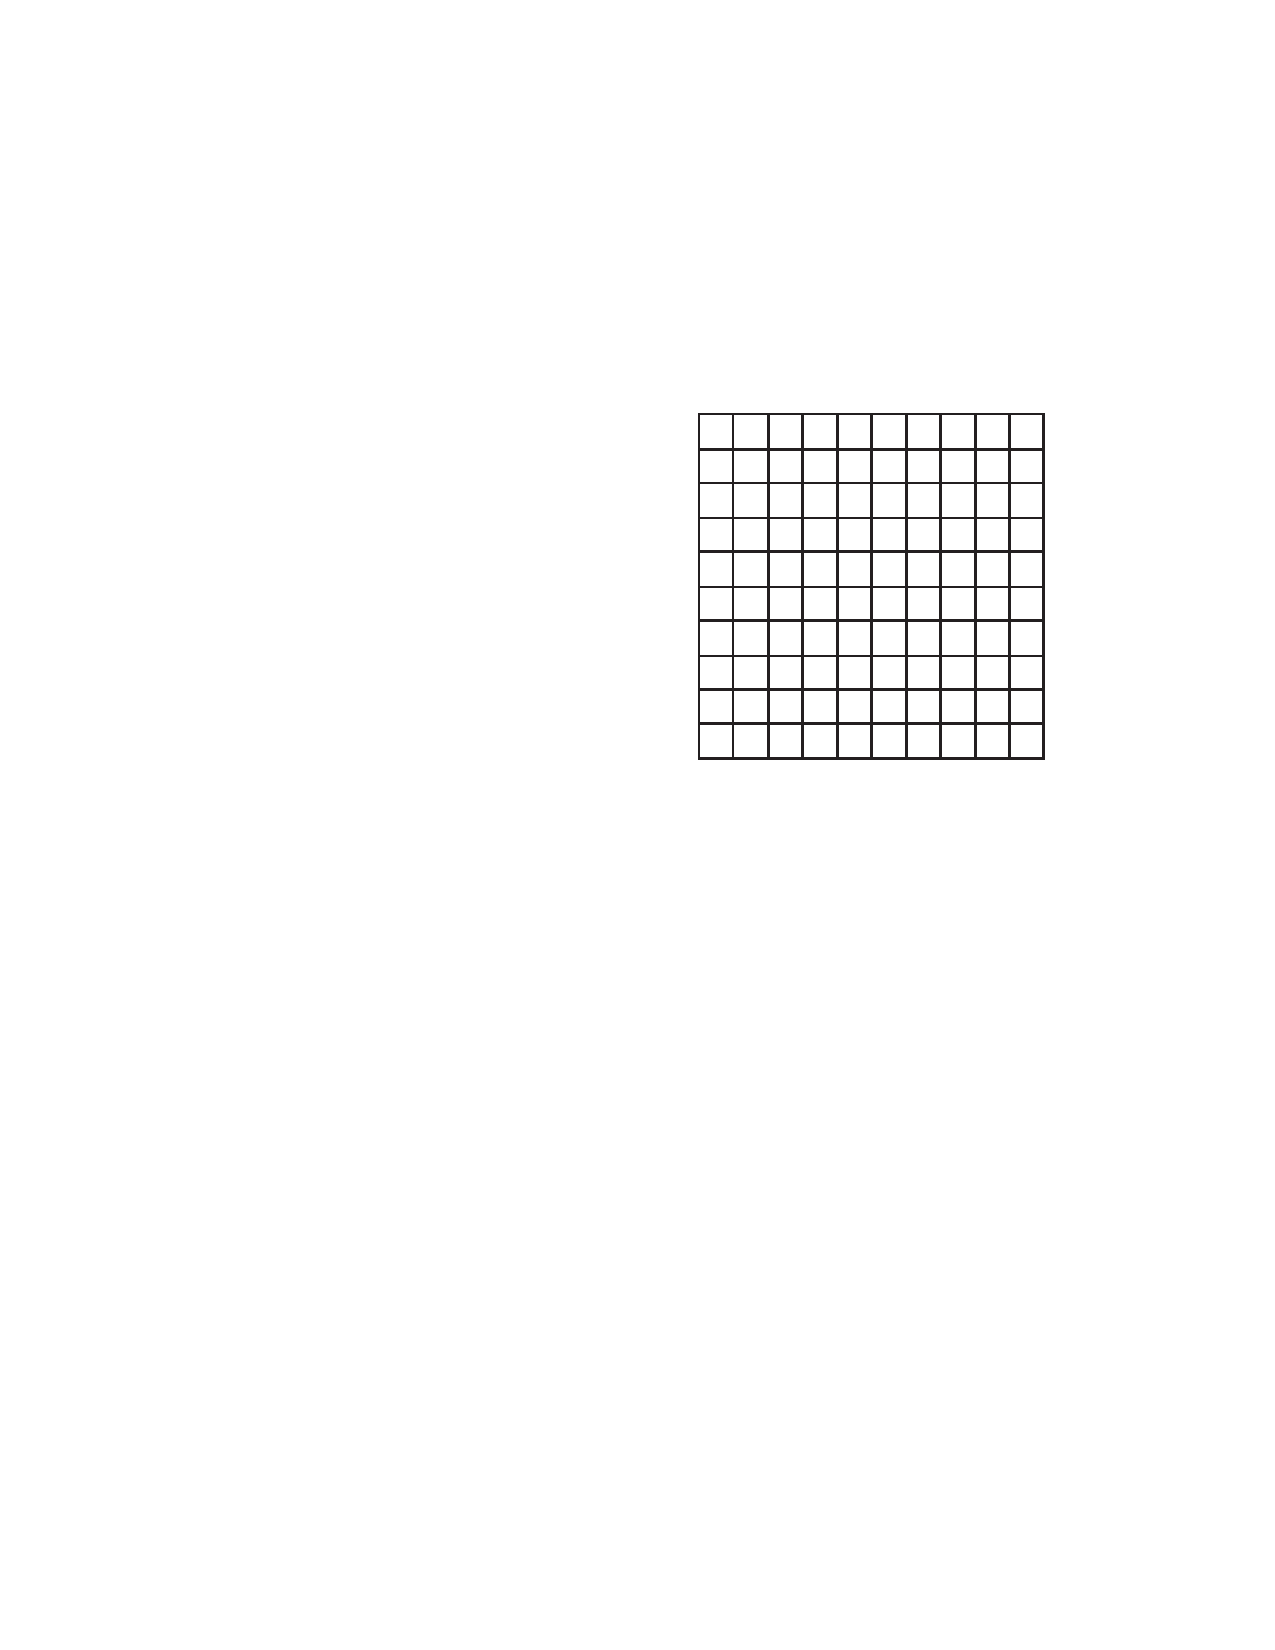
\includegraphics{../graphics/hundredthsGrid}\\

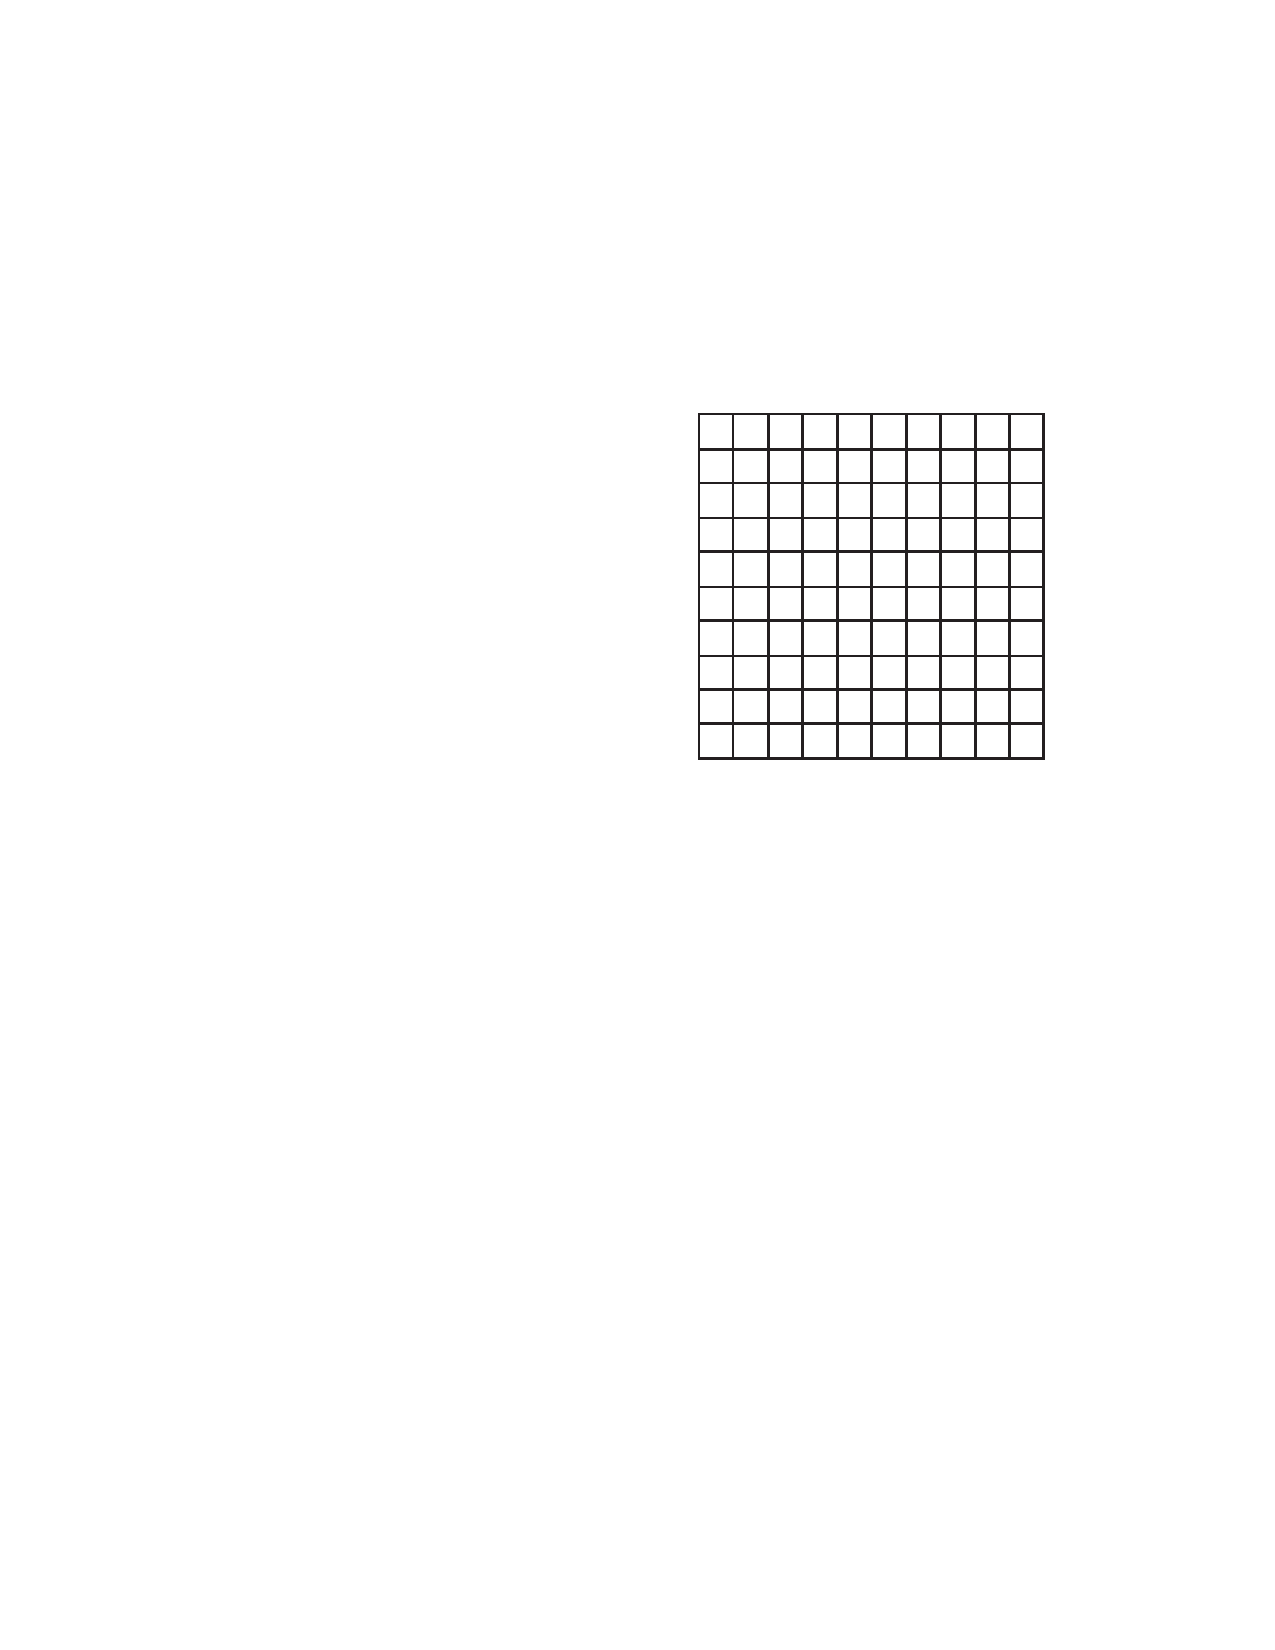
\includegraphics{../graphics/hundredthsGrid}\quad
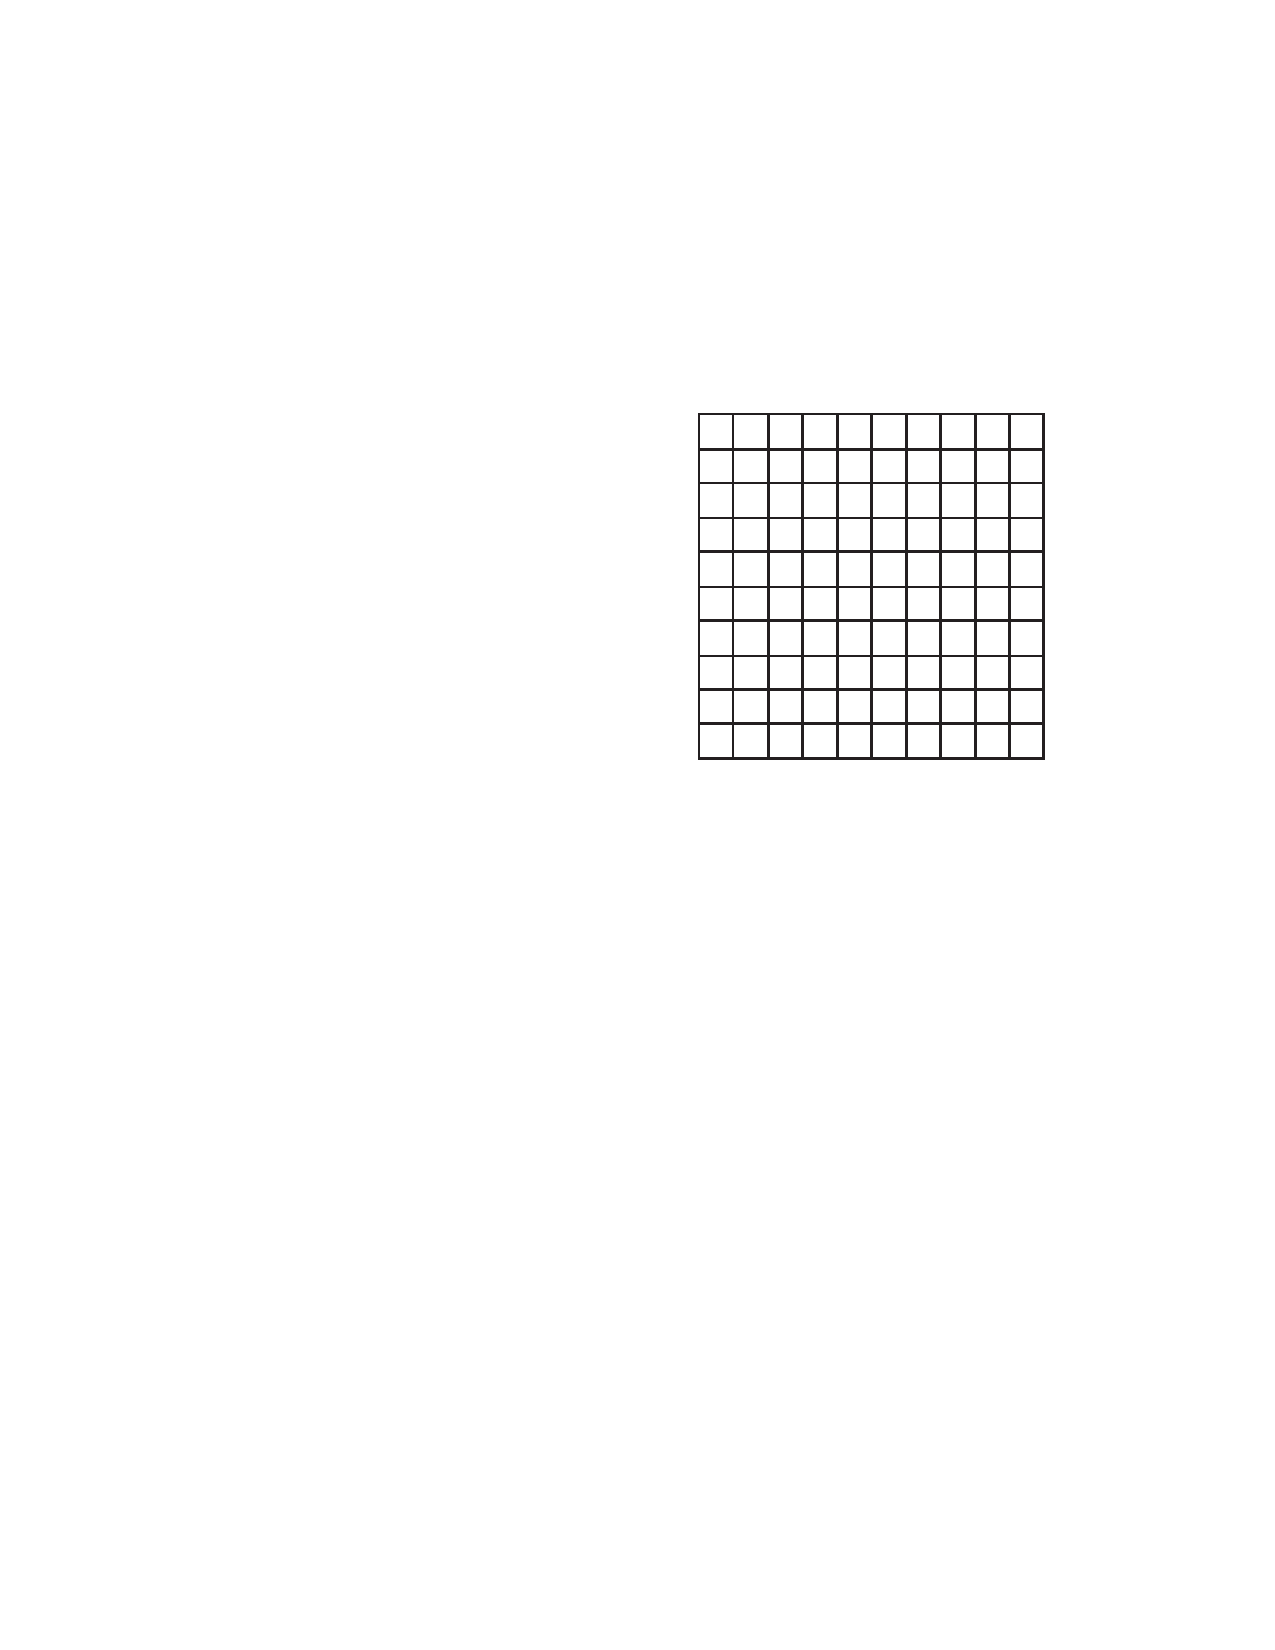
\includegraphics{../graphics/hundredthsGrid}\quad
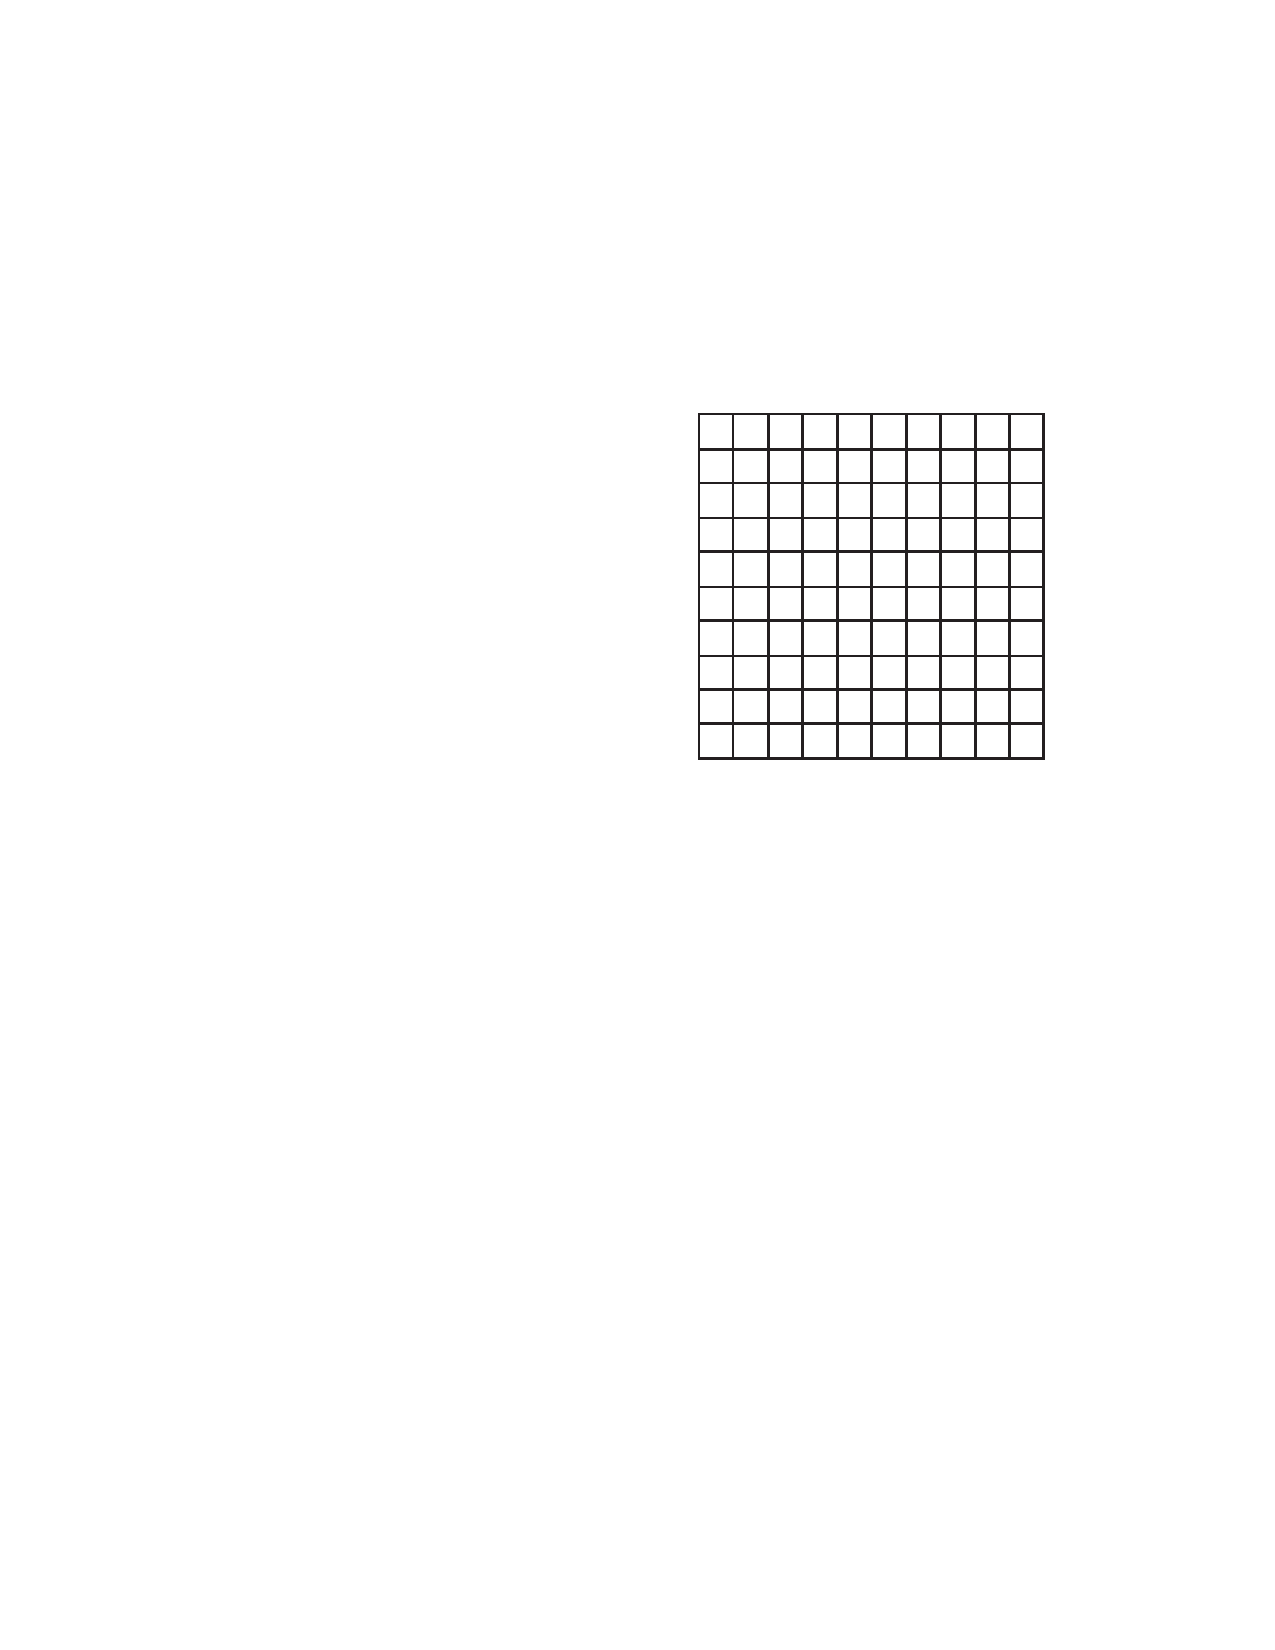
\includegraphics{../graphics/hundredthsGrid}
\end{fullwidth}

\end{prob}



%\newpage
\section{Meanings of Exponents} 

Students in grades 3-7 can use their understanding of counting number arithmetic to build understandings of the arithmetic of negative integers and rational numbers.  Here are the key ideas: 
\begin{quote}
\begin{itemize}
\item The properties of operations (commutative, associative, and distributive properties) are established for counting numbers based on meanings of operations. 
\item As we extend arithmetic to negative integers and rational numbers, we want the properties of operations to continue to hold.  
\end{itemize}
\end{quote}

This activity follows an analogous process for exponents: Students use their understanding of counting number exponents to build an understanding of negative integer and rational exponents.  Here are the key ideas: 
\begin{quote}
\begin{itemize}
\item The rules of exponents are established for counting number exponents based on the meaning of an exponent.  
\item As we extend to negative and rational exponents, we want the rules of exponents to continue to hold.  
\end{itemize}
\end{quote}

\begin{prob}
Students sometimes say that $a^n$ means ``$a$ multiplied by itself $n$ times.''  But for counting number exponents, this is not correct.  For example, how many multiplications are there in $3^5$?  Write a better definition for $a^n$, where $n$ is a counting number.  
\end{prob}

\begin{prob}
Why is $x^3$ not the same function as $3^x$?  We often think of multiplication as ``repeated addition,'' and we find that adding $a$ copies of $b$ gives the same result as adding $b$ copies of $a$.  Does this idea work for thinking of exponentiation as ``repeated multiplication''?  Explain.  
\end{prob}

\begin{prob}
If you do not know (or do not remember) the rules for exponents, you can still use your definition of $a^n$ to figure out other ways of writing expressions with exponents.  Use \textbf{specific values} for letters in expressions of the form $a^na^m$, 
$a^n/a^m$, $(a^n)^m$, and $(ab)^n$ for counting-number exponents, to explain what the rules must be.  Choose specific values that help you explain generally.  
\end{prob}

\begin{prob}
\textbf{Patterns.}  One way to reason about the meanings of zero and negative exponents is to use patterns.  As you complete the following table, \textbf{imagine that you know nothing about zero and negative exponents.}  Instead, use the patterns in the values for positive exponents to reason about what the values should be for zero and negative exponents.  Then reason generally about the meaning of $a^0$ and $a^{-n}$, where $n$ is a counting number and $a$ is a real number.  Are there any values of $a$ for which your reasoning is not valid?  Explain.  
\end{prob}

\begin{minipage}{0.3\textwidth}
\begin{align*}
2^3 &=  \\
2^2 & = \\
2^1 &= \\
2^0 &= \\
2^{-1} &= \\
2^{-2} &= \\
2^{-3} &= \\
\end{align*}
\end{minipage}
\begin{minipage}{0.3\textwidth}
\begin{align*}
3^3 &=  \\
3^2 & = \\
3^1 &= \\
3^0 &= \\
3^{-1} &= \\
3^{-2} &= \\
3^{-3} &= \\
\end{align*}
\end{minipage}
\begin{minipage}{0.3\textwidth}
\begin{align*}
(-2)^3 &=  \\
(-2)^2 & = \\
(-2)^1 &= \\
(-2)^0 &= \\
(-2)^{-1} &= \\
(-2)^{-2} &= \\
(-2)^{-3} &= \\
\end{align*}
\end{minipage}
\begin{minipage}{0.3\textwidth}
\begin{align*}
\left(\frac{1}{2}\right)^3 &=  \\
\left(\frac{1}{2}\right)^2 & = \\
\left(\frac{1}{2}\right)^1 &= \\
\left(\frac{1}{2}\right)^0 &= \\
\left(\frac{1}{2}\right)^{-1} &= \\
\left(\frac{1}{2}\right)^{-2} &= \\
\left(\frac{1}{2}\right)^{-3} &= \\
\end{align*}
\end{minipage}


\begin{prob}
\textbf{Extending the rules.}  A careful way to approach zero and negative integer exponents is to use the rules of exponents (which you established above for counting-number exponents) to determine what 0 and negative integer exponents must mean if the exponent rules continue to hold in this extended domain.
\begin{enumerate}
\item Use the exponent rules to provide two explanations for a sensible definition of $a^0$, being clear about why your definition makes sense.  Note any restrictions on $a$.  
\item Use the exponent rules to provide two explanations for a sensible definition of $a^{-n}$, where $n$ is a counting number.  Again, note any restrictions on $a$.
\end{enumerate}
\end{prob}

\begin{prob}
While trying to decide what $3^{\frac{2}{5}}$ should mean, Katie wondered about the expression $\left(3^{\frac{2}{5}}\right)^5$.  What should Katie's expression be equal to?  Explain, using rules of exponents.  Then use Katie's idea to determine a value for $3^{\frac{2}{5}}$.  
\end{prob}





\newpage
\section{Second Differences}\label{A:secondDifferences}
In a previous activity, we developed strategies for finding the sum of arithmetic series.  In this activity, we use arithmetic series to develop a formula for a sequence that has constant second differences.  Then we demonstrate that all quadratic sequences have constant second differences.  

\begin{prob}
Consider the sequence $f(n)$ given in the table below.  In the rightmost column, $\Delta$ (``delta'') means difference, computed by subtracting the current value of $f(n)$ from the next.  
\vspace{0.1in} 
\[{\renewcommand{\arraystretch}{1.6}
\begin{tabular}{|c|c|c|}\hline
$n$ & $f(n)$ & $\Delta$ \\ \hline
   0     &  \cellcolor{lightgray}4  &  \cellcolor{lightgray}3  \\ \hline
   1     &  7 &   \cellcolor{lightgray}3 \\ \hline
   2     &  10 &  \cellcolor{lightgray}3  \\ \hline
   3     &  13 &  \cellcolor{lightgray}3  \\ \hline
   4     &  16 &  \cellcolor{lightgray}3   \\ \hline
   5     &  19 &    \\ \hline
\rule[5mm]{12mm}{0mm}  &  \rule[5mm]{12mm}{0mm} &\rule[5mm]{12mm}{0mm}    \\ \hline
\end{tabular}}
\]
\vspace{0.1in} 
\begin{enumerate}
\item Explain how $f(5)$ can be computed from the shaded cells in the table.  
\item Generalize your method to develop and explain a formula for $f(n)$.  
\item What was it about the differences that made this problem easy?  
\end{enumerate}
\end{prob}

\newpage

\begin{prob}
Consider the sequence $g(n)$ given in the table below.  
\vspace{0.1in} 
\[{\renewcommand{\arraystretch}{1.6}
\begin{tabular}{|c|c|c|c|}\hline
$n$ & $g(n)$ & $\Delta$ & $\Delta\Delta$ \\ \hline
   0     &  \cellcolor{lightgray}1  &  \cellcolor{lightgray}  & \\ \hline
   1     &  $-2$ &  \cellcolor{lightgray} & \\ \hline
   2     &  1 &  \cellcolor{lightgray}  & \\ \hline
   3     &  10 &  \cellcolor{lightgray} &  \\ \hline
   4     &  25 & \cellcolor{lightgray}  &  \\ \hline
   5     &  46 &   &  \\ \hline
   6     &  73 &   &  \\ \hline
\rule[5mm]{12mm}{0mm}  &  \rule[5mm]{12mm}{0mm} &\rule[5mm]{12mm}{0mm}  &\rule[5mm]{12mm}{0mm}   \\ \hline
\end{tabular}}
\]
\vspace{0.1in} 
\begin{enumerate}
\item Compute $\Delta$ by subtracting the current value of $g(n)$ from the next.  
\item Explain the formula $\Delta(n) = g(n+1)-g(n)$.
\item Check that the shaded cells sum to $g(5)$, and explain how that makes sense based upon how the $\Delta$ values were calculated.  \item Because the $\Delta$ values (``first differences'') are not constant, use the $\Delta\Delta$ column to compute the ``differences of the differences'' (also called ``second differences'').  
\item From the fact that the second differences are constant, develop an explicit formula for $\Delta$ in terms of $n$.  
\end{enumerate}
\end{prob}

\newpage

\begin{prob}
The same sequence $g(n)$ is given below, this time with a formula for $\Delta$ in terms of $n$.    
\vspace{0.1in} 
\[{\renewcommand{\arraystretch}{1.6}
\begin{tabular}{|c|c|c|}\hline
$n$ & $g(n)$ & $\Delta(n)=6n-3$  \\ \hline
   0     &   \cellcolor{lightgray}1  &   \cellcolor{lightgray}$-3$  \\ \hline
   1     &  $-2$ &  \cellcolor{lightgray}3   \\ \hline
   2     &  1 &    \cellcolor{lightgray}9  \\ \hline
   3     &  10 &  \cellcolor{lightgray}15    \\ \hline
   4     &  25 &   \cellcolor{lightgray}21   \\ \hline
   5     &  46 &  27   \\ \hline
   6     &  73 &     \\ \hline
\rule[5mm]{12mm}{0mm}  &  \rule[5mm]{12mm}{0mm} &\rule[5mm]{12mm}{0mm}    \\ \hline
\end{tabular}}
\]
\vspace{0.1in} 
\begin{enumerate}
\item Explain each of the following steps:    
\begin{align*}
g(5) &= 1 + \Delta(0) + \Delta(1) + \Delta(2) + \Delta(3) + \Delta(4)  \\
        &= 1 + (6\cdot 0 -3) + (6\cdot1 -3) + (6\cdot2 -3) + (6\cdot3 -3) + (6\cdot4 -3) \\
        & = 1 + 6\cdot( 0 + 1 + 2 + 3 + 4) + (-3 + -3 + -3 + -3 + -3) \\
        & = 1 + 6\cdot\frac{5\cdot 4}{2} + 5\cdot (-3)
\end{align*}
\item Where do you see arithmetic series in the calculations you just explained?  
\item Generalize the above approach to yield an expression for $g(n)$.  
\item What kind of sequence is $g(n)$?  
\end{enumerate}

\end{prob}

\newpage

\begin{prob}
A general quadratic sequence $h(n)$ is given below.    
\vspace{0.1in} 
\[{\renewcommand{\arraystretch}{1.6}
\begin{tabular}{|c|c|c|c|}\hline
$n$ & $h(n)=an^2+bn+c$ & $\Delta$ & $\Delta\Delta$ \\ \hline
   0     &    &    & \\ \hline
   1     &   &   & \\ \hline
   2     &   &    & \\ \hline
   3     &   &   &  \\ \hline
\rule[5mm]{12mm}{0mm}  &  \rule[5mm]{12mm}{0mm} &\rule[5mm]{30mm}{0mm}  &\rule[5mm]{30mm}{0mm}   \\ \hline
\end{tabular}}
\]
\vspace{0.1in} 
\begin{enumerate}
\item Compute the values of $h(n)$.  
\item Compute $\Delta$ by subtracting the next value of $h(n)$ from the current.  
\item Use the $\Delta\Delta$ column to compute the second differences.  
\item Generalize the result for first differences by computing $\Delta(n)=h(n+1)-h(n)$.
\item Generalize the result for second differences by computing $\Delta\Delta(n)=\Delta(n+1)-\Delta(n)$.
\item Explain how your work demonstrates that, for any quadratic sequence, the second differences must be constant.  
\end{enumerate}
\end{prob}



%\newpage
\section{Integer Addition and Subtraction}\label{A:integerAddition}
In this activity, we explore various models and strategies for 
making sense of addition and subtraction of integers.  

\subsection*{Useful language}
Addition and subtraction problems arise in situations where we add to, take from, put together, 
take apart, or compare quantities.  

Recall that addition and subtraction facts are related.  For example, if we know that $8+5 = 13$, 
then we also know three related facts:  $5+8=13$, $13-8=5$, and $13-5=8$.  In school mathematics, 
these are often called \emph{fact families}.  

\begin{prob}
What are integers?  Describe some situations in which both positive and negative integers arise.  Use the word ``opposite'' in your descriptions.  
\end{prob}

\subsection*{Red and black chips}
\begin{prob}
In a red-and-black-chip model of the integers, red and black chips each count for $1$, but they are opposites, so that they cancel each other out.  Using language from accounting, suppose black chips are assets and red chips are debts.  We add by putting chips together.  Use red and black chips (or draw the letters $R$ and $B$) to model the following computations.
\begin{enumerate}
\item $(-5)+(-3)$
\item $6+(-4)$.
\item $(-7)+9$
\item $2+(-5)$
\end{enumerate}
\end{prob}

\begin{prob}
In the previous problem, you saw different combinations of red and black chips that had the same numerical value.  
\begin{enumerate}
\item How many ways are there to represent $-3$?  Draw two different representations. 
\item Use the phrase ``zero pairs'' to describe how your two representations are related.  
\end{enumerate}
\end{prob}

\begin{prob}
To subtract in the red-and-black-chip model, we can ``take away'' chips, as you might expect.  When we don't have enough
chips of a particular color, we can always add ``zero pairs.''  Use this idea to model the following subtraction problems: 
\begin{enumerate}
\item $6-8$
\item $4-(-3)$
\item $(-6)-5$
\item $(-3)-(-7)$
\end{enumerate}
\end{prob}

\subsection*{Subtraction as missing addend}
\begin{prob}
To evaluate a subtraction expression, we can solve a related addition equation.  For example, $11-7$ is the solution to $7+\rule[-2pt]{12pt}{.5pt} =11$.  Use this idea to evaluate the subtraction expressions in the previous problem.  
\end{prob}

\subsection*{Subtraction as difference on the number line}
\begin{prob}
Use a number line to reason about $b-a$ by asking how to get from $a$ to $b$:  How far?  And in which direction?   For example, to evaluate $11-7$, we can ask how to get from $7$ to $11$.  We travel $4$ units to the right.  Use this idea to evaluate the subtraction expressions in the previous problems.
\end{prob}

\begin{prob}
How is subtraction different from negation?  
\end{prob}

\begin{prob}
Use what you have learned to explain why $a-(-b)=a+b$.  
\end{prob}

\subsection*{Other Models}  
Use the following models for addition and subtraction of integers.  Each model requires two decisions:  (1) how positive and negative integers are `opposite' in the situation, and (2) how addition and subtraction are `opposite' in a different way.  
\begin{itemize}
\item A postal carrier who brings checks and bills---and who also takes them away.  
\item Walking on an North-South number line, facing either North or South, and walking either forward or backward.  
\end{itemize}


%\newpage
\section{Integer Multiplication}\label{A:integerMultiplication}



In this activity, we explore various models and strategies for 
making sense of multiplication of integers.  

\subsection*{Continuing patterns}
\begin{prob}
\begin{enumerate}
\item Continue the following patterns, and explain why it makes sense to continue them in that way.    

\begin{minipage}{0.45\textwidth}
\begin{align*}
4\times 3 &= 12 \\
4\times 2 &= \\
4\times 1 &= \\
4\times 0 &= \\
4\times (-1) &= \\
4\times (-2) &= \\
4\times (-3) &= \\
\end{align*}
\end{minipage}
\begin{minipage}{0.45\textwidth}
\begin{align*}
3\times 6 &= 18 \\
2\times 6 &= \\
1\times 6 &= \\
0\times 6 &= \\
(-1)\times 6 &= \\
(-2)\times 6 &= \\
(-3)\times 6 &= \\
\end{align*}
\end{minipage}
\begin{minipage}{0.45\textwidth}
\begin{align*}
(-7)\times 3 &= -21 \\
(-7)\times 2 &= \\
(-7)\times 1 &= \\
(-7)\times 0 &= \\
(-7)\times (-1) &= \\
(-7)\times (-2) &= \\
(-7)\times (-3) &= \\
\end{align*}
\end{minipage}

\item What rule of multiplication might a student infer from the first pattern? 
\item What rule of multiplication might a student infer from the second pattern?
\item What rule of multiplication might a student infer from the third pattern?
\end{enumerate}
\end{prob}

\subsection*{Using properties of operations}

\begin{prob}
Suppose we \emph{do not know} how to multiply negative numbers but we do know that $4\times 6=24$. We will use this fact and the properties of operations to reason about products involving negative numbers.  
\begin{enumerate}
\item What do we know about $A$ and $B$ if $A+B=0$?  
\item Use the distributive property to show that the expression $4\times 6 + 4\times(-6)$ is equal to $0$.  
Then use that fact to reason about what $4\times(-6)$ should be.  
\item Use the distributive property to show that the expression $4\times (-6) + (-4)\times (-6)$ is equal to $0$.  
Then use that fact to reason about what $(-4)\times(-6)$ should be.  
\end{enumerate}
\end{prob}

\subsection*{Walking on a number line}
\begin{teachingnote}
Again there are two decisions to make: (1) distinguishing positive and negative for the multiplicand; (2) distinguishing positive and negative for the multiplier.
\end{teachingnote}
\begin{prob} 
Matt is a member of the Ohio State University
  Marching Band. Being rather capable, Matt can take $x$ steps of size
  $y$ inches for all integer values of $x$ and $y$.  If $x$ is
  positive it means \textit{face North and take $x$ steps.} If $x$ is
  negative it means \textit{face South and take $|x|$ steps.} If $y$
  is positive it means your step is a \textit{forward step of $y$
    inches.} If $y$ is negative it means your step \textit{is a
    backward step of $|y|$ inches.}
\begin{enumerate}
\item Discuss what the expressions $x \cdot y$ means in this
  context. In particular, what happens if $x = 1$? What if $y=1$?
\item If $x$ and $y$ are both positive, how does this fit with the ``repeated addition'' model of multiplication?    
\item Using the context above and specific numbers, 
demonstrate the general rule:
\[
\text{negative}\cdot \text{positive} = \text{negative}
\]
Clearly explain how your problem shows this.
\item Using the context above and specific numbers, 
demonstrate the general rule:
\[
\text{positive}\cdot \text{negative} = \text{negative}
\]
Clearly explain how your problem shows this.\item Using the context above and specific numbers, 
demonstrate the general rule:
\[
\text{negative}\cdot \text{negative} = \text{positive}
\]
Clearly explain how your problem shows this.
\end{enumerate}
\end{prob}


%\newpage
\section{Divisibility Statements}\label{A:divisibilityStatements}

Let $a|b$ mean $b=aq$ for some integer $q$.  (Read $a|b$ as ``$a$ divides $b$''.)  

\begin{prob}
Using the numbers 56 and 7, make some true statements using the notation above and one or more of the words factor, multiple, divisor, and divides.  
\end{prob}

\begin{prob}
Use the definition of \emph{divides} to decide which of the following are true and which are false.  If a statement is true, find $q$ satisfying the definition of divides.  If it is false, give an explanation.  (Hint:  Try to reason about multiplication rather than using your calculator.)
\begin{enumerate}
\item $21|2121$
\item $3|(9\times 41)$
\item $6|(2^4\times 3^2\times 7^3\times 13^5)$
\item $100000|(2^3\times 3^9\times 5^{11}\times 17^8)$
\item $6000|(2^{21}\times 3^7 \times 5^{17}\times 29^5)$
\item $p^3q^5r|(p^5q^{13}r^7s^2t^{27})$
\item $7|(5\times 21 + 14)$
\end{enumerate}
\end{prob}

\fixnote{Need some easier examples above.  Below, we need at least one that isn't true.  Use converses of some of these?}

\begin{prob}
If $a|b$ and $a|c$ does $a|(bc)$?  Explain. 
\end{prob}

\begin{prob}
If $a|b$ and $a|c$ does $a|(b+c)$?  Explain.  
\end{prob}

\begin{prob}
If $a|(b+c)$ and $a|c$ does $a|b$?  Explain.  
\end{prob}

\begin{prob}
Suppose that $$(3^5\cdot 7^9\cdot 11^x\cdot 13^y)|(3^a\cdot 7^b\cdot 11^{19}\cdot 13^7)$$
What values of $a$, $b$, $x$, and $y$ make true statements? 
\end{prob}

%\newpage
\section{Fraction Multiplication}\label{A:fractionMultiplication}

\begin{prob}
Suppose $x$ and $y$ are counting numbers.  
\begin{enumerate}
\item What is our convention for the meaning of $xy$ as repeated addition?  
\item In our convention for the meaning of the product $xy$, which letter describes 
\emph{how many groups} and which letter describes \emph{how many in one group}? 
\item In the product $xy$, the $x$ is called the \emph{multiplier} and $y$ is called the \emph{multiplicand}.  
Use these words to describe the meaning of $xy$ as repeated addition. 
\end{enumerate}
\end{prob}

\vspace{1in}

\begin{prob}
In the Common Core State Standards, fractions and fraction operations are built from \emph{unit fractions}, which are fractions with a $1$ in the numerator.  The meaning of a fraction $\frac{a}{b}$ involves three steps: (1) determining the whole; (2) describing the meaning of $\frac{1}{b}$; and (3) describe the meaning of the fraction $\frac{a}{b}$.  Use pictures to illustrate these three steps for the fraction
$\frac{3}{5}$.  
\end{prob}

\vspace{1in}

\begin{prob}
Now we combine the ideas from the previous two problems to describe meanings for simple multiplication of fractions.  
\begin{enumerate}
\item Without computing the result, describe the meaning of the product $5 \times \frac{1}{3}$.
\item Without computing the result, describe the meaning of the product $\frac{1}{3}\times 5$.
\item Without using the commutativity of multiplication (which we have not established for fractions), 
use these meanings and pictures to explain what the products should be. 
\end{enumerate}
\end{prob}

\vspace{1in}

\subsection*{Area Models}
\begin{prob}
Beginning with a unit square, use an area model to illustrate the following:  
\begin{enumerate}
\item $\frac{1}{3}\times \frac{1}{4}$ 
\item $\frac{7}{3}\times \frac{5}{4}$
\end{enumerate}
\end{prob}

\vspace{1.5in}
\
\begin{prob}
When computing $2\frac{1}{3}\times 3\frac{2}{5}$, Byron says that the answer is $6\frac{2}{15}$.  
\begin{enumerate}
\item Explain Byron's method. 
\item How do you know that he is incorrect?  
\item Use what is right about his method to show what he is missing. 
\end{enumerate}
\end{prob}

%\newpage
\section{Arithmetic Series}\label{A:arithmeticSeries}

In this activity, we explore \emph{arithmetic series}, which are sums of consecutive terms from an arithmetic sequence.

Ms. Nguyen's math class has been looking at ``triangular numbers.''  The first 6 triangular numbers are shown below. 
\[
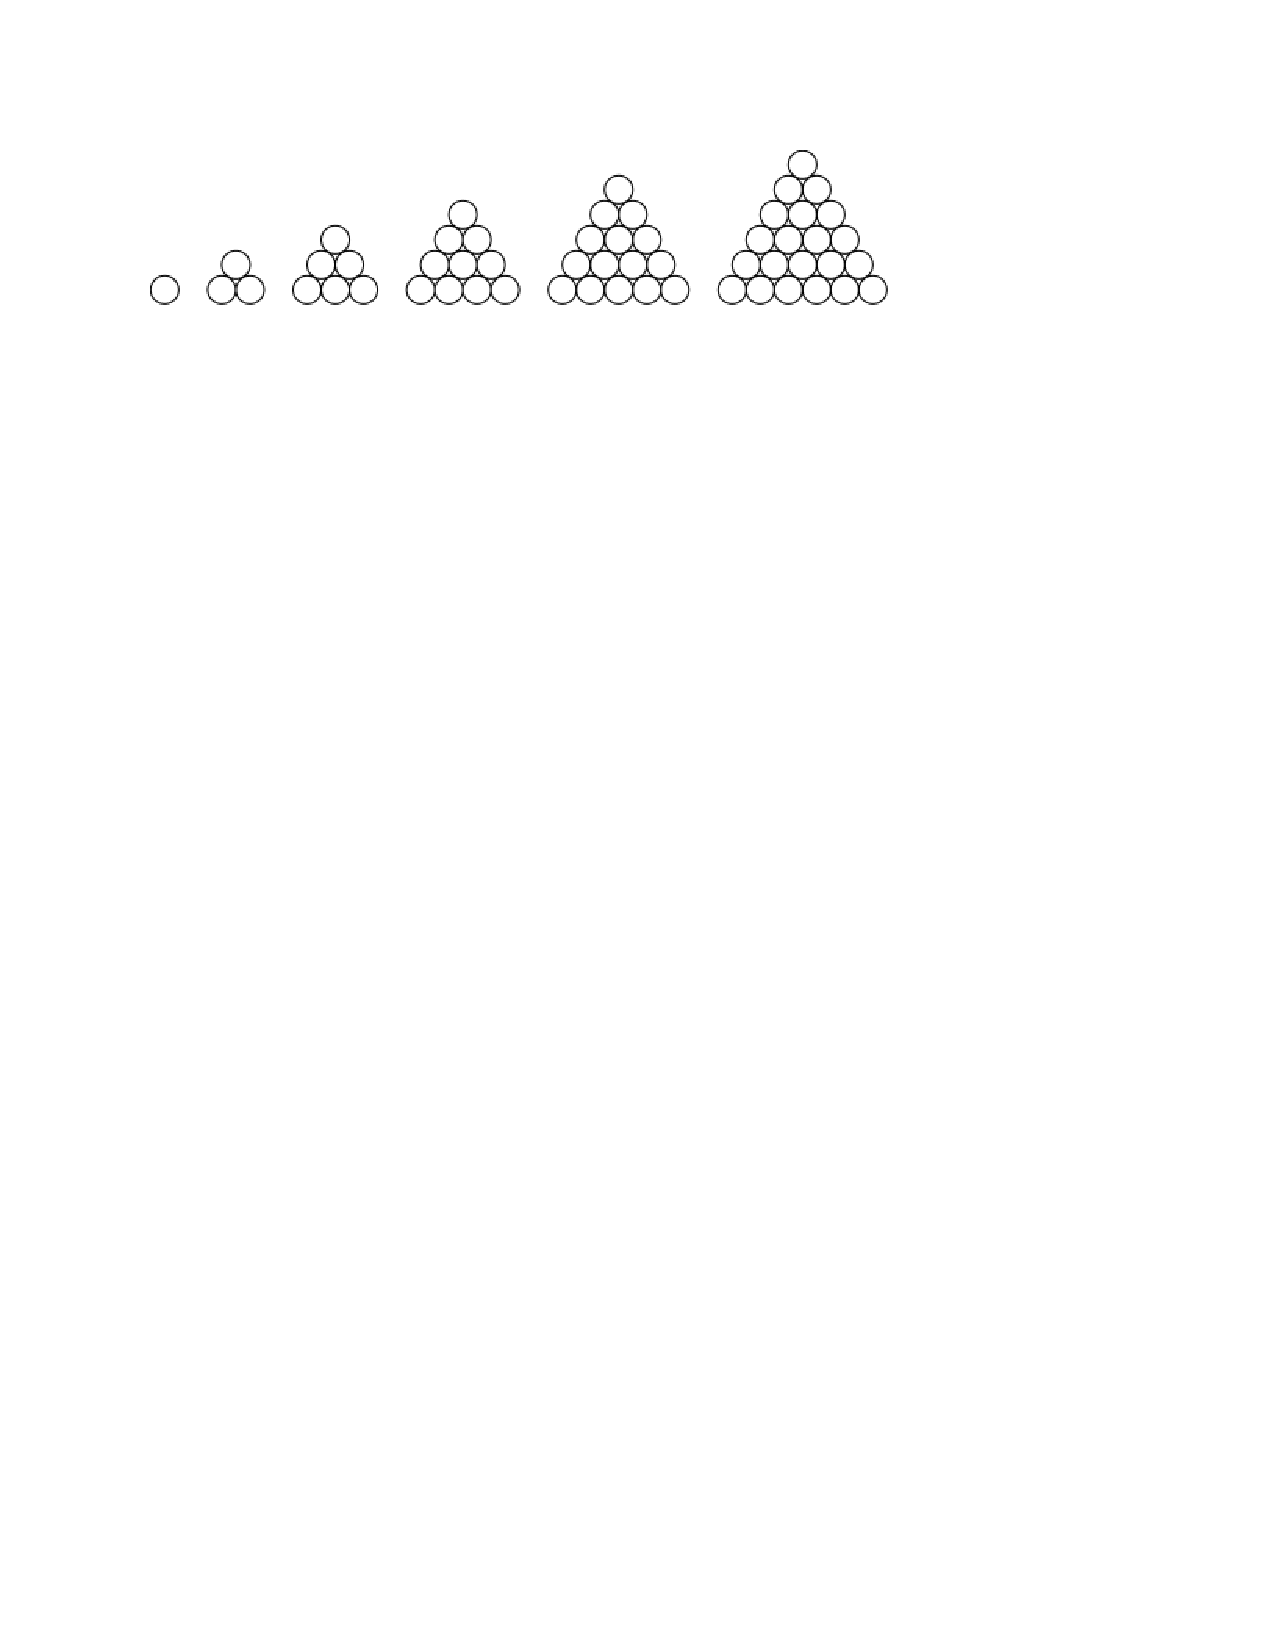
\includegraphics{../graphics/triangularNumbers}
\]
\fixnote{Need an original graphic here.}

\begin{prob}
Blair wanted to find the $551^{st}$ triangular number.  She used a table and looked for a pattern in the \emph{sequence of partial sums}:  $1, 1+2, 1+2+3, \dots$.  Help her finish her idea.  
\end{prob}

\begin{prob}
Kaley realized the the $551^{st}$ triangular number would be the sum 
\[
1+2+3+4+\dots+548+549+550+551
\]
She started pairing the first with the last number; the second with the second-to-last; the third with the third-to-last; and so on.  She saw that the averages are always the same.  Help her finish her idea.  
\end{prob}

\begin{prob}
Ali begin by writing out the sum forward and backward and follows:  
\[
\begin{array}{c@{ + }c@{ + }c@{ + }c@{ + }c@{ + }c@{ + }c@{ + }c@{ + }c@{ + }c@{ + }c@{ + }c@{ + }c}
1 & 2 & 3 & 4 & 5 & 6 & \cdots & 546 & 547 & 548 & 549 & 550 & 551 \\
551 & 550 & 549 & 548 & 547 & 546 & \cdots & 6 & 5 & 4 & 3 & 2 & 1 
\end{array}
\]
Help her finish her idea.  Be sure to explain clearly what happens ``in the dots.''  Does it matter whether there are an even or an odd number of terms?  
\end{prob}

\begin{prob}
Cooper was interested in a different triangular number and drew the following picture:   
\[
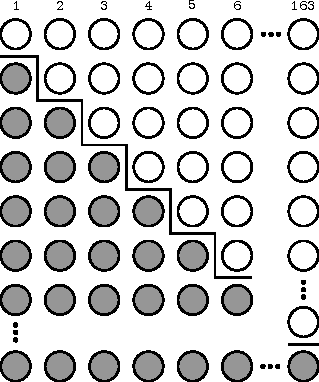
\includegraphics{../graphics/sum1.pdf}
\]
Which triangular number was he finding?  Help him finish his idea.  Be sure to explain clearly what 
happens ``in the dots.'' 
\end{prob}


\begin{prob}
Sum the numbers:  
\[
106 + 112 + 118 + \dots + 514
\]
\end{prob}

\begin{prob}
Sum the numbers:
\[
2.2 + 2.9 + 3.6 + 4.3 + \dots + 81.3
\]
\end{prob}


\begin{prob}
Suppose you have an arithmetic sequence beginning with $a$, with a constant difference of $d$ and with $n$ terms.  
\begin{enumerate}
\item What is the $n^{th}$ term of the sequence?  
\item Use dots to write the series consisting of the first $n$ terms of this sequence.
\item Find the sum of this series.  
\end{enumerate}
\end{prob}



%\newpage
\section{Geometic Series}\label{A:geometicSeries}

In this activity, we explore \emph{geometric series}, which are sums of consecutive terms from an geometric sequence.

Ms. Radigan's math class has been trying to compute the following sums:  
$$1+2+4+8+\dots+2^{19}$$
$$\frac{2}{3}+\frac{2}{9}+\frac{2}{27}+\dots+\frac{2}{3^{13}}$$

\begin{prob}
Kelsey used tables and looked for pattern in the \emph{sequence of partial sums}:  $1, 1+2, 1+2+4, \dots$.  Help her finish her idea for both sequences.    
\end{prob}

\begin{prob}
For the sum beginning with $\frac{2}{3}$, Erin started by drawing a large square (which she imagined as having area 1), and she shaded in $\frac{2}{3}$ of it.  Then she shaded in $\frac{2}{9}$ more, and so on.  Help her finish her idea.  
\end{prob}

\begin{prob}
Ryan wrote out all of the terms in the first sum, represented as powers of 2, beginning with $1+2+2^2+2^3$.  
Then he realized that because the terms formed a geometric sequence, he could multiply the series by the common ratio of 2, and the resulting series would be almost identical to the first, differing only at the beginning and the end.  By subtracting the first series from the second, all of the middle terms would cancel.  Help him finish his idea.  
\end{prob}

\begin{prob}
Ali said, ``Here is a thought experiment.  I take a sheet of paper, rip it perfectly into thirds, place one piece to start a pile that I will call A, another piece to start a pile I will call B, and I keep the third piece in my hands.  I then rip that piece into thirds, place one piece on pile A, one piece on pile B, and keep the third.  Notice that each of pile A and pile B have $\frac{1}{3}+\frac{1}{9}$ of a sheet of paper, and I still have $\frac{1}{9}$ of a sheet in my hands.  I continue this process until I place $\frac{1}{3^{13}}$ of a sheet on each pile and still have $\frac{1}{3^{13}}$ of a sheet in my hands.  

Help Ali finish her idea.  
\end{prob}


\begin{prob}
Sum the expression:  
\[
\frac{2}{3}+\frac{4}{9}+\frac{8}{27}+\dots+\frac{2^n}{3^n}
\]
What happens to this sum as $n$ gets really large?  
\end{prob}


\begin{prob}
Consider the expression: 
$$\frac{7}{10}+\frac{7}{100}+\frac{7}{1000}+\dots+\frac{7}{10^n}$$
\begin{enumerate}
\item Find the sum of the expression. 
\item What happens to this sum as $n$ gets really large?  
\item How does this help you explain why a particular repeating decimal is a particular rational number?  Be sure to indicate what repeating decimal and what rational number you are talking about.  
\end{enumerate}
\end{prob}


\begin{prob}
Suppose you have an geometric sequence beginning with $a$, with a constant ratio of $r$ and with $n$ terms.  
\begin{enumerate}
\item What is the $n^{th}$ term of the sequence?  
\item Use dots to write the series consisting of the first $n$ terms of this sequence.
\item Find the sum of this series.  
\end{enumerate}
\end{prob}



%\newpage
\section{Solving Quadratics}\label{A:solvingQuadratics}
\fixnote{Separate into two activities.  This is too much for one day.  Aim to complete through problem 8 on day 1.}
Here we explore various methods for solving quadratic equations in one variable.  \textbf{Please read all instructions carefully.}

\begin{prob}
Is $\sqrt{4}=\pm 2$?  Explain. 
\end{prob}

\vfill

\begin{teachingnote}
Both $2$ and $-2$ are ``square roots'' of $4$ because $2^2=4$ and $(-2)^2=4$, and both of them are solutions to the equation $x^2=4$.  The question is whether the radical symbol refers to both of them, either of them (you choose?), or a specific one of them.  
\end{teachingnote}

\begin{prob}
Suppose that $\sqrt{4}=\pm 2$?  Then evaluate $\sqrt{4}+\sqrt{9}$.  
\end{prob}

\begin{teachingnote}
$$\sqrt{4}+\sqrt{9}=\pm2+\pm3=5, -1, 1, or -5$$
\end{teachingnote}

\vfill

\begin{prob}
What does your calculator say about $\sqrt{4}+\sqrt{9}$?  
\end{prob}

\vfill 

\begin{teachingnote}
Now emphasize the conventional meaning of the radical symbol:  For $a>0$ then $\sqrt{a}$ means the positive square root of $a$.  
\end{teachingnote}



\begin{prob}
In the following problems, you \textbf{may not use the quadratic formula}.  But just for the record, write down the quadratic formula.  
\end{prob}
\begin{teachingnote}
Many students will write only $\frac{-b\pm\sqrt{b^2-4ac}}{2a}$, but we want them to write the following:  

$$\text{If }ax^2+bx+c=0\text{ and }a\ne 0\text{, then }x=\frac{-b\pm\sqrt{b^2-4ac}}{2a}\text{.}$$
Note that if the radical symbol were to refer to both a positive and negative square root, then there would be no reason to write $\pm$ outside the radical symbol.  
\end{teachingnote}

\vfill

\newpage

\begin{prob}
In the following list of equations, solve those that are \textbf{easy} to solve.  
\begin{enumerate}
\item $(x-3)(x+2)=0$
\item $(x-3)(x+2)=1$
\item $(2x-5)(3x+1)=0$
\item $(x-a)(x-b)=0$
\item $(x-1)(x-3)(x+2)(2x-3)=0$
\end{enumerate}
\end{prob}

\begin{prob}
Regarding the previous problem, state the property of numbers that made all but one of the equations easy to solve.  
\end{prob}

\begin{teachingnote}
Zero product property:  If $ab = 0$ then $a=0$ or $b=0$.  Note that this doesn't work when the right side is not 0.  
\end{teachingnote}

\vspace{0.3in}


%\begin{prob} For each part below, write a linear equation with the state solution.  
%\begin{enumerate}
%\item $x=\frac{2}{3}$
%\item $x=\frac{a}{b}$
%\end{enumerate}
%\end{prob}

\begin{prob}For each part below, write a quadratic equation with the stated solution(s) and no other solutions.  
\begin{enumerate}
\item $x=7$ or $x=-4$
\item $x=p$ or $x=q$
\item $x=3$
\item $x=\frac{1\pm\sqrt{5}}{2}$
 \end{enumerate}
\end{prob}

\begin{teachingnote}
In the following problem, discuss ways of explaining that 
$$\pm\sqrt{\frac{1}{2}}=\pm\frac{1}{\sqrt{2}}=\pm\frac{\sqrt{2}}{2}$$
\end{teachingnote}

\begin{prob}
In the following list of equations, solve those that are \textbf{easy} to solve.  
\begin{enumerate}
\item $x^2=5$
\item $x^2 - 4 = 2$
\item $x^2 - 4x = 2$
\item $2x^2=1$
\item $(x-2)^2=5$
\end{enumerate}
\end{prob}
\vspace{0.3in}

\begin{prob}
Regarding the previous problem, state the property of numbers that made all but one of the equations easy to solve.  
\end{prob}
\vspace{0.3in}

\begin{teachingnote}
If $u^2=a$ then $u=\pm\sqrt{a}$.
\end{teachingnote}

\begin{prob}
Although $160$ is not a square in base ten, what could you add to $160$ so that the result would be a square number?  
\end{prob}

\begin{prob}
 Consider the polynomial expression $x^2+6x$ to be a number in base $x$.  We want to add to this polynomial so that the result is a square in base $x$.  
\begin{enumerate}
\item Use ``flats'' and ``longs'' to draw a picture of this polynomial as a number in base $x$, adding enough ``ones'' so that you can arrange the polynomial into a square.  
\vspace{0.5in}
\item What ``feature'' of the square does the new polynomial expression represent?  
\item Why does it make sense to call this technique ``completing the square''? 
\item Use your picture to help you solve the equation $x^2+6x=5$.  
\end{enumerate}
\end{prob}

\newpage

\begin{prob}
Complete the square to solve the following equations: 
\begin{enumerate}
\item $x^2+3x=4$
\vspace{.8in}
\item $x^2+bx=q$
\vspace{.8in}
\item $2x^2+8x=12$
\vspace{.8in}
\item $ax^2+bx+c=0$
\vspace{.8in}
\end{enumerate}  
\end{prob}

\fixnote{Perhaps delete the rest of the problems or move them elsewhere.}
\begin{prob}
Find all solutions to $x^3-3x^2+x+1=0$.  Hint:  One solution is $x=1$.  
\end{prob}

\begin{prob}
Solve the following equation
\[
x^5 - 4x^4 - 18x^3 + 64x^2 + 17x -60 = 0
\]
assuming you know that $1$, $-1$, and $3$ are roots.
\end{prob}


%\newpage
\section{Solving Cubic Equations}\label{A:solvingCubics}

To solve the cubic equation $x^3+px+q=0$, we use methods that were discovered and advanced by various mathematicians, including Ferro, Tartaglia, and Cardano.  The approach is organized in three steps.  \textbf{Make notes in the margin as you follow along.}  

%\begin{itemize}
%\item Step 1:  Replace $x$ with $u+v$.
%\item Step 2: Set $uv$ so that all of the terms are eliminated except for $u^3$, $v^3$, and constant terms.
%\item Step 3: Clear denominators, recognize the equation as a quadratic in $u^3$, and use the quadratic formula.
%\end{itemize}

\subsection{Step 1:  Replace $x$ with $u+v$}
In $x^3+px+q=0$, let $x = u + v$.  % $$(u+v)^3+p(u+v)+q=0.$$ 
Show that the result can be written as follows:  

$$u^3+v^3+(3uv+p)(u+v)+q = 0.$$

\subsection{Step 2: Set $uv$ to eliminate terms}
If $3uv+p=0$, then all of the terms are eliminated except for $u^3$, $v^3$, and constant terms. Explain why the equation simplifies nicely to:

$$u^3+v^3 + q = 0.$$

Solve $3uv+p=0$ for $v$, substitute, and show that we have:  

$$u^3+\left( \frac{-p}{3u}\right)^3+q=0.$$

\subsection{Step 3:  Recognize the equation as a quadratic in $u^3$ and solve}

By multiplying by $u^3$, show that we get a quadratic in $u^3$:   

$$u^6+qu^3+\left( \frac{-p}{3}\right)^3 = 0.$$

Show that this has solutions: 

$$u^3 = \frac{-q\pm\sqrt{q^2-4\left( \frac{-p}{3}\right)^3}}{2}.$$

Now, use the facts $v= -p/(3u)$ and $x = u + v$ to write a formula for $x$: 

$$x = \sqrt[3]{\frac{-q\pm\sqrt{q^2-4\left( \frac{-p}{3}\right)^3}}{2}} 
+  \frac{-p}{3\sqrt[3]{\frac{-q\pm\sqrt{q^2-4\left( \frac{-p}{3}\right)^3}}{2}}}.$$

\begin{prob}
How many values does this formula give for $x$?  From the original equation $x^3+px+q=0$, how many solutions should we expect? 
\end{prob}
\vfill

\begin{prob}
Use the above formula to solve the specific equation $x^3-15x-4=0$.  Show that $$x = \sqrt[3]{2 \pm \sqrt{-121}} + \frac{5}{\sqrt[3]{2\pm\sqrt{-121}}}.$$
Are these values of $x$ real numbers?  
\end{prob}
\vfill


\begin{prob}
Use technology to graph $y=x^3-15x-4$.  According to the graph, how many real roots does the polynomial have?  What is going on?  
\end{prob}
\vfill

\begin{prob}
Choose ``plus'' in the $\pm$, and check that $2+\sqrt{-1}$ is a cube root of $2 + \sqrt{-121}$.  Use that fact to simplify the above expression for $x$.  What do you notice?  
\end{prob}
\vfill

\begin{prob}
Now choose ``minus'' in the $\pm$ above, and find the value of $x$.  What do you notice?  
\end{prob}

\vfill
In both cases, the formula requires computations with square roots of negative numbers, but the result is a real solution.  These kinds of occurrences were the historical impetus behind the gradual acceptance of complex numbers.  



\end{document}
